%!TeX root=20_Hauptteil.tex

\chapter{Versuchsdurchführung und Evaluation}
\label{cap:versuchsdurchführung}
Dieses Kapitel beschreibt die praktische Durchführung der Versuche und die Auswertung der Ergebnisse.
Es baut auf den in den Kapiteln~\ref{cap:implementierung_kartierung} und~\ref{cap:implementierung_positionsbestimmung} beschriebenen Implementierungen auf und gliedert sich in die beiden Teilaufgaben Kartierung und Positionierung.
Beide werden zunächst in ihrer Durchführung und anschließend in ihrer Evaluation behandelt.
Als externer Computer wird ein Lenovo ThinkPad mit einem Intel~Core~i5-1145G7 (11.~Generation), $16\,\text{GB}$ 
Arbeitsspeicher und integrierter Intel~Iris~Xe-Grafik unter Ubuntu~24.04 genutzt.




\section{Durchführung und Evaluation der Kartierung}
\label{sec:durchfuehrung_kartierung}
Dieser Abschnitt beschreibt, wie die physische Karte angefertigt und in der Versuchsumgebung angebracht wird.
Anschließend wird das Vorgehen zum Aufzeichnen und erstellen der digitalen Karte beschrieben.
Im Letzten Teil wird die Qualität und das Vorgehen der Kartierung bewertet.

\subsection{Erstellen und Anbringen der physischen Karte}
\label{sec:anbringen_karte}
Zunächst wurde die digitale Sollkarte konstruiert und aus ihr eine druckfähige Datei abgeleitet.
Der Entwurf ist so angelegt, dass drei nebeneinander ausgelegte Teile die zusammenhängende Karte bilden.
Als Trägermaterial für die Teilstücke dient eine 1,3~m breite, matte Klebefolie.
Jede dieser Bahnen trägt aufgedruckte Markierungen, die eine lagerichtige Ausrichtung der Bögen zueinander sicherstellen.
Die Bahnen weisen eine Länge von jeweils 5,0~m auf, woraus sich für die vollständige Karte eine Ausdehnung von $5{,}0$~m~$\times$~$3{,}9$~m ergibt.

Hauptbestandteil der Karte sind die aufgedruckten AprilTags der Familie \texttt{tag36h11}.
Insgesamt kommen vier verschiedene Markergrößen zum Einsatz: 0,170~m, 0,300~m, 1,0~m und 0,12~m.
Geplottet werden 68 Fiducial-Marker der Größe 0,170~m, 24 Fiducial-Marker der Größe 0,300~m sowie vier Fiducial-Marker der Größe 1,0~m.
Die Größe 0,12~m ist nur ein einziges Mal (\gls{id}~1) vorhanden und dient dem Starten des \gls{uav}s.
Bei dem Start wären die anderen Fiducial-Marker zu groß, sodass die Bodenkamera sie nicht vollständig erfassen könnte und zu Beginn keine Lokalisierung möglich wäre.

Die Anordnung und Größe der Fiducial-Marker ist so gewählt, dass bei einer Flughöhe von 1,0~m stets mindestens zwei Fiducial-Marker im Sichtfeld liegen.
Eine Ausnahme bilden die Eckbereiche, in denen die dort platzierten großformatigen Fiducial-Marker das Sichtfeld bereits weitgehend ausfüllen.
Um das Zentrum herum sind die Fiducial-Marker in einem geringeren Abstand zueinander, um bei einer niedrigeren Flughöhe ausreichend Detektionen zu erhalten. 

In Abbildung~\ref{fig:tag_karte_oic} die angebrachte Karte dargestellt.
Der Fiducial-Marker zum starten des \gls{uav}s ist im geometrischen Zentrum der Karte rot markiert. 
Der Ursprung der Karte und des Weltkoordinatensystems liegt leicht versetzt zum Zentrum.
Der Fiducial-Marker mit der \gls{id}~0 definiert diesen Ursprung und ist grün umrandet.

\begin{figure}[htbp]
    \centering
    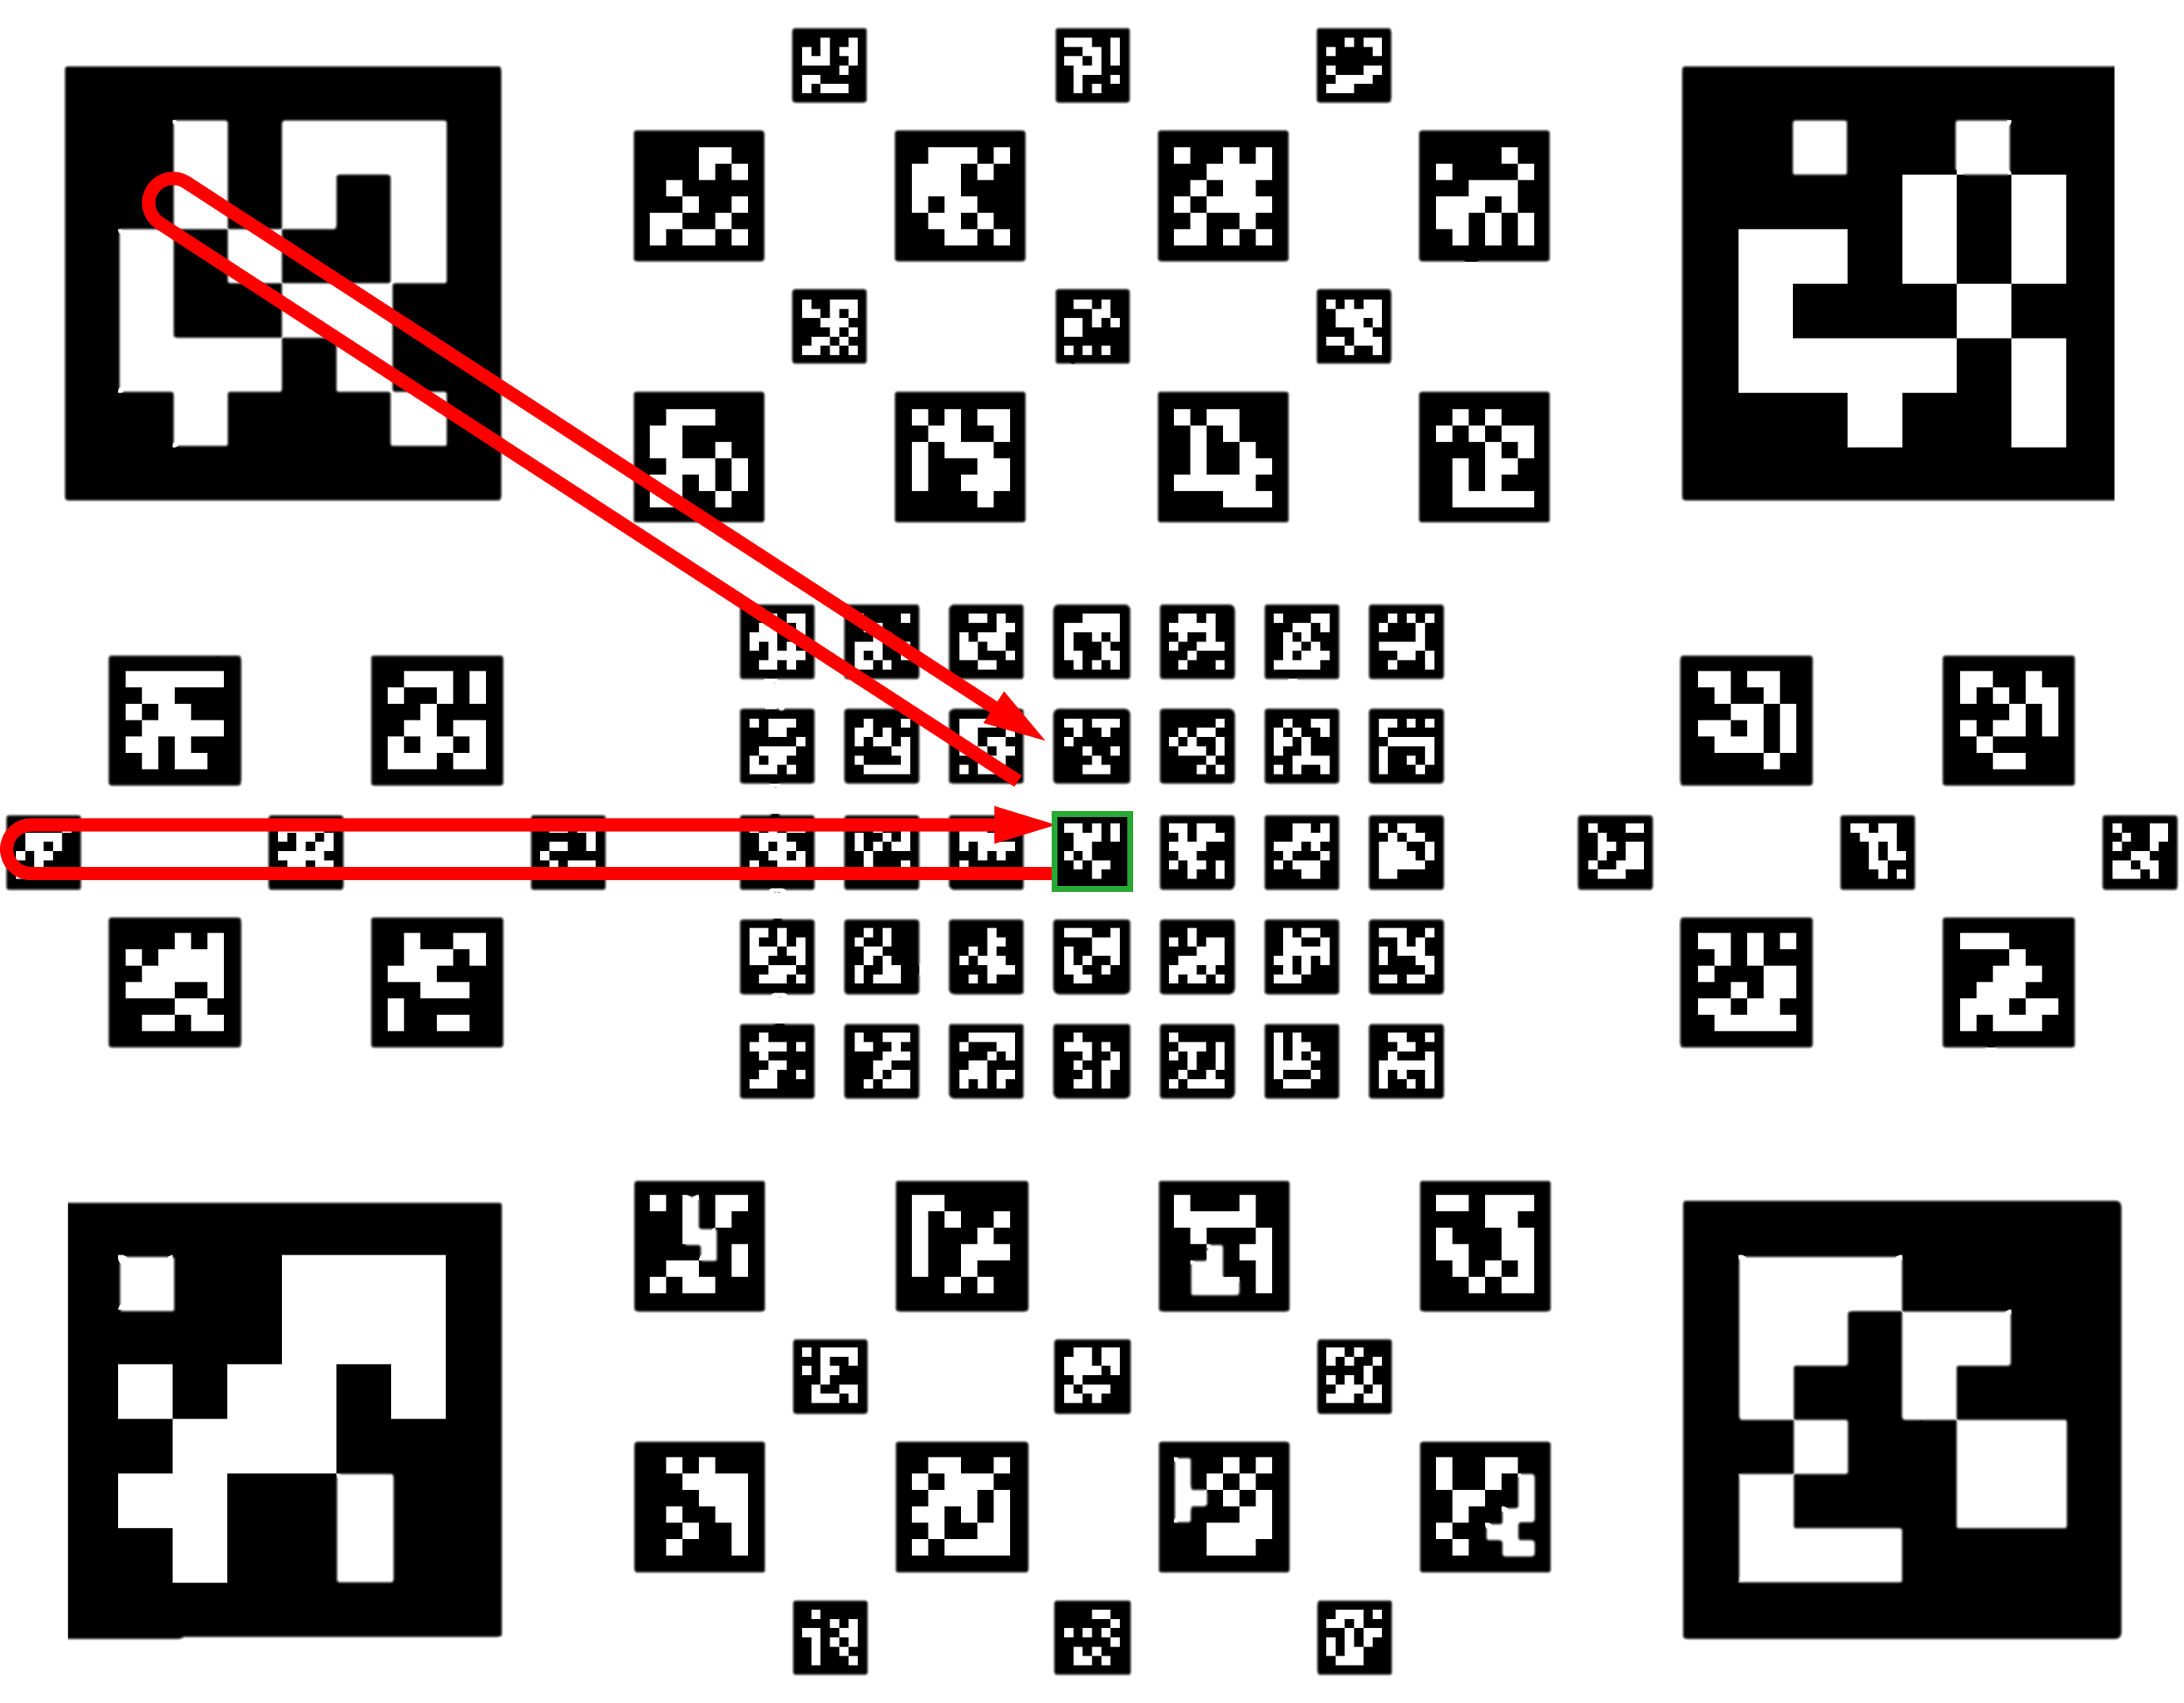
\includegraphics[width=0.76\textwidth]{Bilder/Karte_mit_Pfeilen.png}
    \caption{Tag-Karte der OIC-Flughalle. Der Kartenursprung (Tag~0) ist grün umrandet, die roten Pfeile zeigen exemplarisch das sternförmige Abgehen zur Erzeugung von Loop-Closures.}
    \label{fig:tag_karte_oic}
\end{figure}
\FloatBarrier

Die Versetzung des Markers mit der \gls{id}~0 gegenüber dem geometrischen Zentrum ist bewusst gewählt.
Das Zentrum ist bereits durch den Startmarker mit einer Kantenlänge von 0,120~m belegt, der als einziger Anker der Kartierung eine vergleichsweise kleine Bezugsfläche und damit eine ungenauere Lagebestimmung böte.
Der Ursprung liegt daher auf dem benachbarten Fiducial-Marker der gängigen Größe von 0,170~m. 

Beim Aufbringen der Klebefolie auf den Boden der Versuchsumgebung wurde besonderes Augenmerk auf eine exakte Ausrichtung gelegt.
Dennoch lässt sich zwischen den Zentren der Eckmarker mit den Kennungen 200 bis 203 ein Versatz von etwa $5$~mm messen.
Der Versatz entlang der Bahnrichtung, also zwischen den Markern 200 und 201 beziehungsweise 202 und 203, ist darauf zurückzuführen, dass sich die Folie nach dem Abziehen der Trägerschicht geringfügig zusammengezogen hat.
Der Versatz zwischen den Markern 200 und 203 beziehungsweise 201 und 202 resultiert aus der großen Bahnlänge und der damit verbundenen erschwerten Handhabung beim Anbringen der Karte.

Die digitale Konstruktion der Karte liefert unmittelbar eine Referenz mit bekannten Sollwerten, deren Genauigkeit durch die genannten Abweichungen nach oben begrenzt ist.
Diese Referenz wird im folgenden als Ground Truth bezeichnet.



\subsection{Aufzeichnung und Kartenerstellung}
\label{sec:aufnahme_karte}
Die eigentliche Aufzeichnung der physischen Karte erfolgt wie in Abschnitt \ref{sec:ablauf_kartierung} beschrieben, in drei Schritten auf dem externen Computer.
Dabei entsteht zunächst ein \gls{ros2}-Bag, während die Kamera (Logitech C922) von Hand über die Karte geführt wird.
Die Kamera arbeitet mit 15~\gls{fps} und einer Auflösung von 1920~$\times$~1080.

Entscheidend beim Führen der Kamera ist eine möglichst senkrechte Ausrichtung zum Boden sowie eine hohe Zahl gleichzeitig erfasster Marker.
Jeder Fiducial-Marker muss im Verlauf der Aufnahme mindestens einmal erfasst werden, da nur beobachtete Fiducial-Marker in die Karte eingehen.
Besondere Aufmerksamkeit erfordern dabei die Eckmarker, deren große Kantenlänge eine vollständige Erfassung im Bild erschwert.

Die Kameraführung folgt einem sternförmigen Muster, verläuft also vom Mittelpunkt der Karte aus in Richtung der Ränder und anschließend wieder zurück.
Das wiederholte Abgehen der Karte in verschiedenen Richtungen erzeugt Loop-Closure-Constraints, welche die spätere Optimierung der Karte verbessern.
Zum Ende der Aufnahme führt der Weg einmal um die Karte herum, um dort ebenfalls ein Loop-Closure-Constraint zu erzeugen.
Insgesamt umfasst das aufgezeichnete Material eine Dauer von 166~Sekunden, was bei 15~\gls{fps} rund 13,9~\gls{gb} entspricht.

\subsection*{Offline Fiducial-Marker Detektion}
\label{sec:sync_and_detect}
Der erste Bag wird nach \ref{sec:offline_detektion_apriltags} dem Node \texttt{sync\_and\_detect\_node} übergeben, der die Fiducial-Marker detektiert und die Zeitstempel synchronisiert.
Aus der Aufnahme des ersten Schritts wurden 2390 Frames der Kameraaufzeichnung untersucht und dabei 46443 Fiducial-Marker detektiert.
Dieser Bag bildet die Eingangsgröße für die eigentliche Kartenerstellung mit Tag\gls{slam}.




\subsubsection*{Optimierung und Parametrierung von TagSLAM.}
\label{sec:parametrierung_tagslam}
Der Bag aus der Offline-Detektion wird mit dem Node \texttt{tagslam\_from\_bag} verarbeitet.
Dabei wird der Fall einer unbekannten Karte zugrunde gelegt, in der keinerlei Vorwissen über die Lage der Fiducial-Marker vorliegt.

Die Kartierung erfolgt in drei Versuchen mit unterschiedlicher Parametrierung.
Ziel ist es, eine Parametrierung zu ermitteln, die sich künftig zur Kartierung unbekannter 
Umgebungen eignet und dabei einen tragfähigen Kompromiss zwischen Rechenaufwand und Genauigkeit bietet.
Alle Läufe verarbeiten denselben Detektions-Bag und unterscheiden sich ausschließlich in der Parametrierung von TagSLAM.
Die wichtigsten Parameter der jeweiligen Läufe können Tabelle~\ref{tab:tagslam_params} entnommen werden.
Nicht aufgeführte Parameter wurden entsprechend den Vorgabewerten aus der TagSLAM-Dokumentation gesetzt.
\begin{table}[htbp]
\centering
\begin{tabular}{lccc}
\toprule
\textbf{Parameter} & \textbf{Versuch~1} & \textbf{Versuch~2} & \textbf{Versuch~3} \\
\midrule
\texttt{optimizer\_mode}            & \texttt{fast} & \texttt{fast} & \texttt{slow} \\
\texttt{max\_subgraph\_error}       & $50$            & $10$            & $10$ \\
\texttt{max\_num\_incremental\_opt} & $50$          & $10$          & $50$ \\
\texttt{Fixierung der Marker}                & keine         & $z$, $\varphi_x$, $\theta_y$ & $z$, $\varphi_x$, $\theta_y$\\
\midrule
\texttt{minimum\_viewing\_angle}                & \multicolumn{3}{c}{$15{,}0$} \\
\texttt{minimum\_tag\_area}                     & \multicolumn{3}{c}{$2500$} \\
\texttt{use\_approximate\_sync}                 & \multicolumn{3}{c}{\texttt{true}} \\
\bottomrule
\end{tabular}
\caption[Parametrierung der drei Versuche]{Parametrierung der drei Versuche.}
\label{tab:tagslam_params_laeufe}
\end{table}
\FloatBarrier



\subsubsection*{Versuch~1:}
Der erste Versuch dient allein der schnellen Gewinnung einer Startschätzung, weshalb der Parameter \texttt{optimizer\_mode} auf \texttt{fast} gesetzt ist.
Die Schwelle \texttt{max\_subgraph\_error} bleibt mit $50$ tolerant, da einzelne fehlerhafte Messungen die angestrebte grobe Schätzung nicht wesentlich beeinträchtigen.
Ebenso ist \texttt{max\_num\_incremental\_opt} mit $50$ hoch angesetzt, sodass der Faktorgraph nur selten vollständig optimiert wird.
Es wird außer dem Ursprungsmarker keine weitere Fixierung vorgenommen, sodass sich die restlichen Fiducial-Marker anhand von Fiducial-Marker 0 optimieren.
Der Mindestbetrachtungswinkel \texttt{minimum\_viewing\_angle} von $15{,}0$ stellt sicher, dass nur hinreichend senkrecht erfasste Fiducial-Marker in die Optimierung eingehen.
Durch den Parameter \texttt{minimum\_tag\_area} wird festgelegt, dass zu klein dargestellte Fiducial-Marker nicht in die Optimierung einfließen.
Die näherungsweise zeitliche Zuordnung über \texttt{use\_approximate\_sync} ist aktiviert, um abweichende Zeitstempel zwischen den Nachrichten des Bags auszugleichen.



\subsubsection*{Versuch~2:}
Der zweite Versuch übernimmt gemeinsame Einstellungen aus Versuch eins und nutzt zusätzlich das aus der vorherigen Optimierung gewonnene Wissen.
Um fehlerhafte Messungen von der Karte fernzuhalten, wird die Schwelle \texttt{max\_subgraph\_error} auf $10$ herabgesetzt.
Zugleich sinkt \texttt{max\_num\_incremental\_opt} auf $10$, wodurch der Faktorgraph häufiger vollständig optimiert wird und die Lösung an Genauigkeit gewinnt.

Da alle Fiducial-Marker flach auf dem Boden und damit in derselben Ebene wie der Ursprung liegen, wird ihre Höhe mit $z=0$ vorgegeben und über ein sehr kleines \texttt{position\_noise} in $z$ von $10^{-6}$ fixiert.
Ebenso werden die Verkippungen um die $x$- und $y$-Achse auf $0$ gesetzt und über ein \texttt{rotation\_noise} von $10^{-6}$ in diesen beiden Achsen fixiert.
Die verbleibenden Freiheitsgrade, also die Lage in der $x$-$y$-Ebene und die Drehung um die $z$-Achse, bleiben schätzbar, werden jedoch über \texttt{position\_noise} in $x$ und $y$ von $0{,}2$ schwach an die übernommene Startlage gebunden.
Der grundsätzliche Aufbau dieser Fixierung ist in Quellcode~\ref{lst:tagslam_tag_noise} für die Kennungen 0 bis 2 dargestellt.
\begin{lstlisting}[caption={Tagweise Fixierung der Markerlagen in \texttt{tagslam.yaml}},label={lst:tagslam_tag_noise},captionpos=b]
tags:
  - id: 0
    size: 0.170
    pose:
      position: {x: 0.0, y: 0.0, z: 0.0}
      rotation: {x: 0.0, y: 0.0, z: 0.0}
    position_noise: {x: 1.0e-06, y: 1.0e-06, z: 1.0e-06}
    rotation_noise: {x: 1.0e-06, y: 1.0e-06, z: 1.0e-06}
  - id: 1
    size: 0.120
    pose:
      position: {x: -0.242321, y: -0.000951, z: 0.0}
      rotation: {x: 0.0, y: 0.0, z: -0.000313}
    position_noise: {x: 0.4, y: 0.4, z: 1.0e-06}
    rotation_noise: {x: 1.0e-06, y: 1.0e-06, z: 0.5}
  - id: 2
    size: 0.170
    pose:
      position: {x: -0.241930, y: 0.241503, z: 0.0}
      rotation: {x: 0.0, y: 0.0, z: -0.001375}
    position_noise: {x: 0.4, y: 0.4, z: 1.0e-06}
    rotation_noise: {x: 1.0e-06, y: 1.0e-06, z: 0.5}
\end{lstlisting}


\subsubsection*{Versuch~3:}
Der dritte Versuch behält die Einstellungen des zweiten weitgehend bei, wechselt jedoch in den Betriebsmodus \texttt{slow}, um die Genauigkeit weiter zu steigern.
Um die Rechenzeit dabei nicht ausufern zu lassen, wird \texttt{max\_num\_incremental\_opt} wieder auf $50$ angehoben, sodass der Graph seltener vollständig optimiert wird.
Die Schwelle \texttt{max\_subgraph\_error} verbleibt bei $10$.

Wie der zweite Lauf übernimmt der dritte die im ersten Versuch geschätzten Positionen als Startlagen und bindet 
alle Fiducial-Marker über $z$=0 sowie die auf 0 gesetzten Verkippungen um die $x$- und $y$-Achse an die Bodenebene.

Aufgrund der positiven Ergebnisse und der hohen Laufzeit im Betriebsmodus \texttt{slow} wurde auf einen Vergleichslauf mit \texttt{fast} verzichtet.

\subsection{Evaluation der Kartierung}
\label{sec:evaluation_kartierung}
Als Grundlage der Qualität der Kartierung dient die Ground Truth. 
Verglichen werden die Abweichungen der Markerzentren in der Kartenebene.





Von den 97 aufgebrachten Markern erfassen die Karten aller drei Versuche jeweils 96.
Der Fiducial-Marker mit der Kennung 202 fehlt in allen Fällen, da er augenscheinlich während der Aufzeichnung nicht erfasst wurde.
Es handelt sich um einen der Eckmarker mit einer Kantenlänge von 1,0~m, für dessen vollständige Abbildung im Bild ein entsprechend großer Abstand zum Boden erforderlich ist.
Als Grund ist eine Fehlerhafte Aufzeichnung im ersten Bag zu nennen. 
Dieser Fiducial-Marker wurde nicht sorgfältig genug bei der Aufnahme des Bags betrachtet.

Nachfolgende Abbildungen zeigen den Aufgenommenen Karten aus der Draufsicht und vergleicht diese mit dem Ground Truth.
\begin{figure}[htbp]
    \centering
    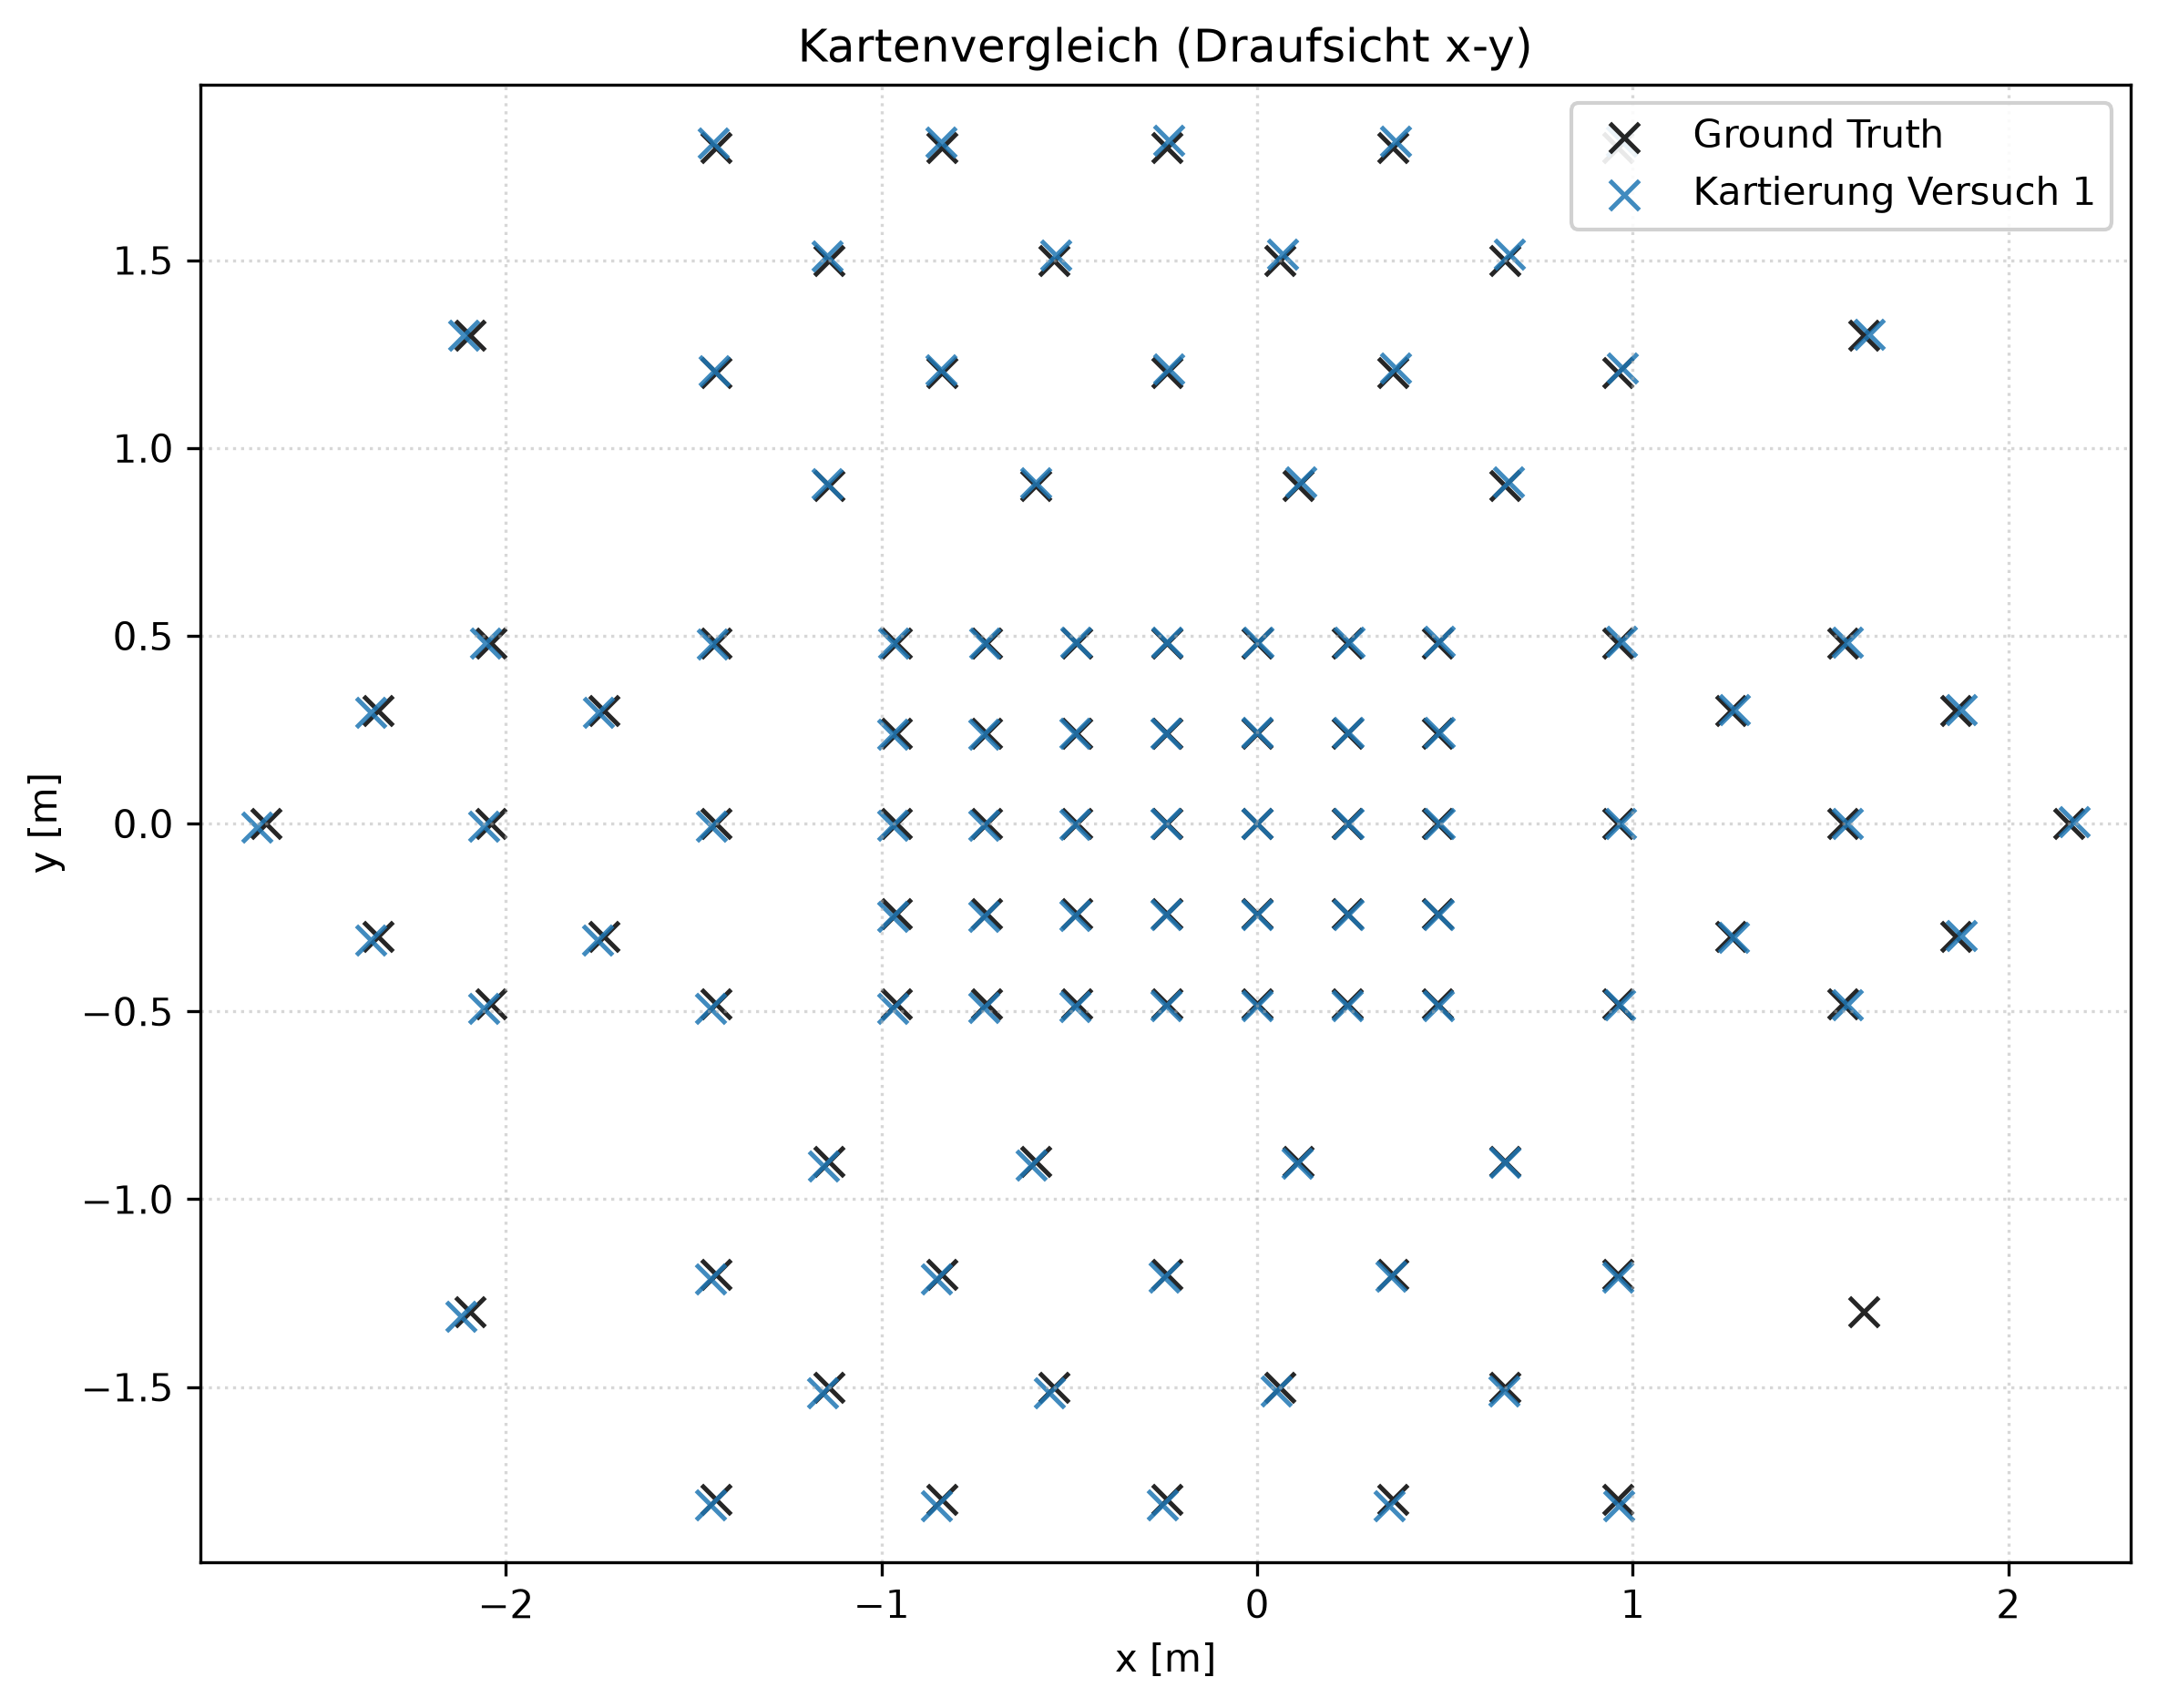
\includegraphics[width=0.7\textwidth]{Bilder/karten_vergleich_ueberlagert_versuch_1.png}
    \caption{Überlagerung der in Versuch~1 erzeugten Karte mit der Ground Truth}
    \label{fig:kartenvergleich_versuch1}
\end{figure}
\FloatBarrier

\begin{figure}[htbp]
    \centering
    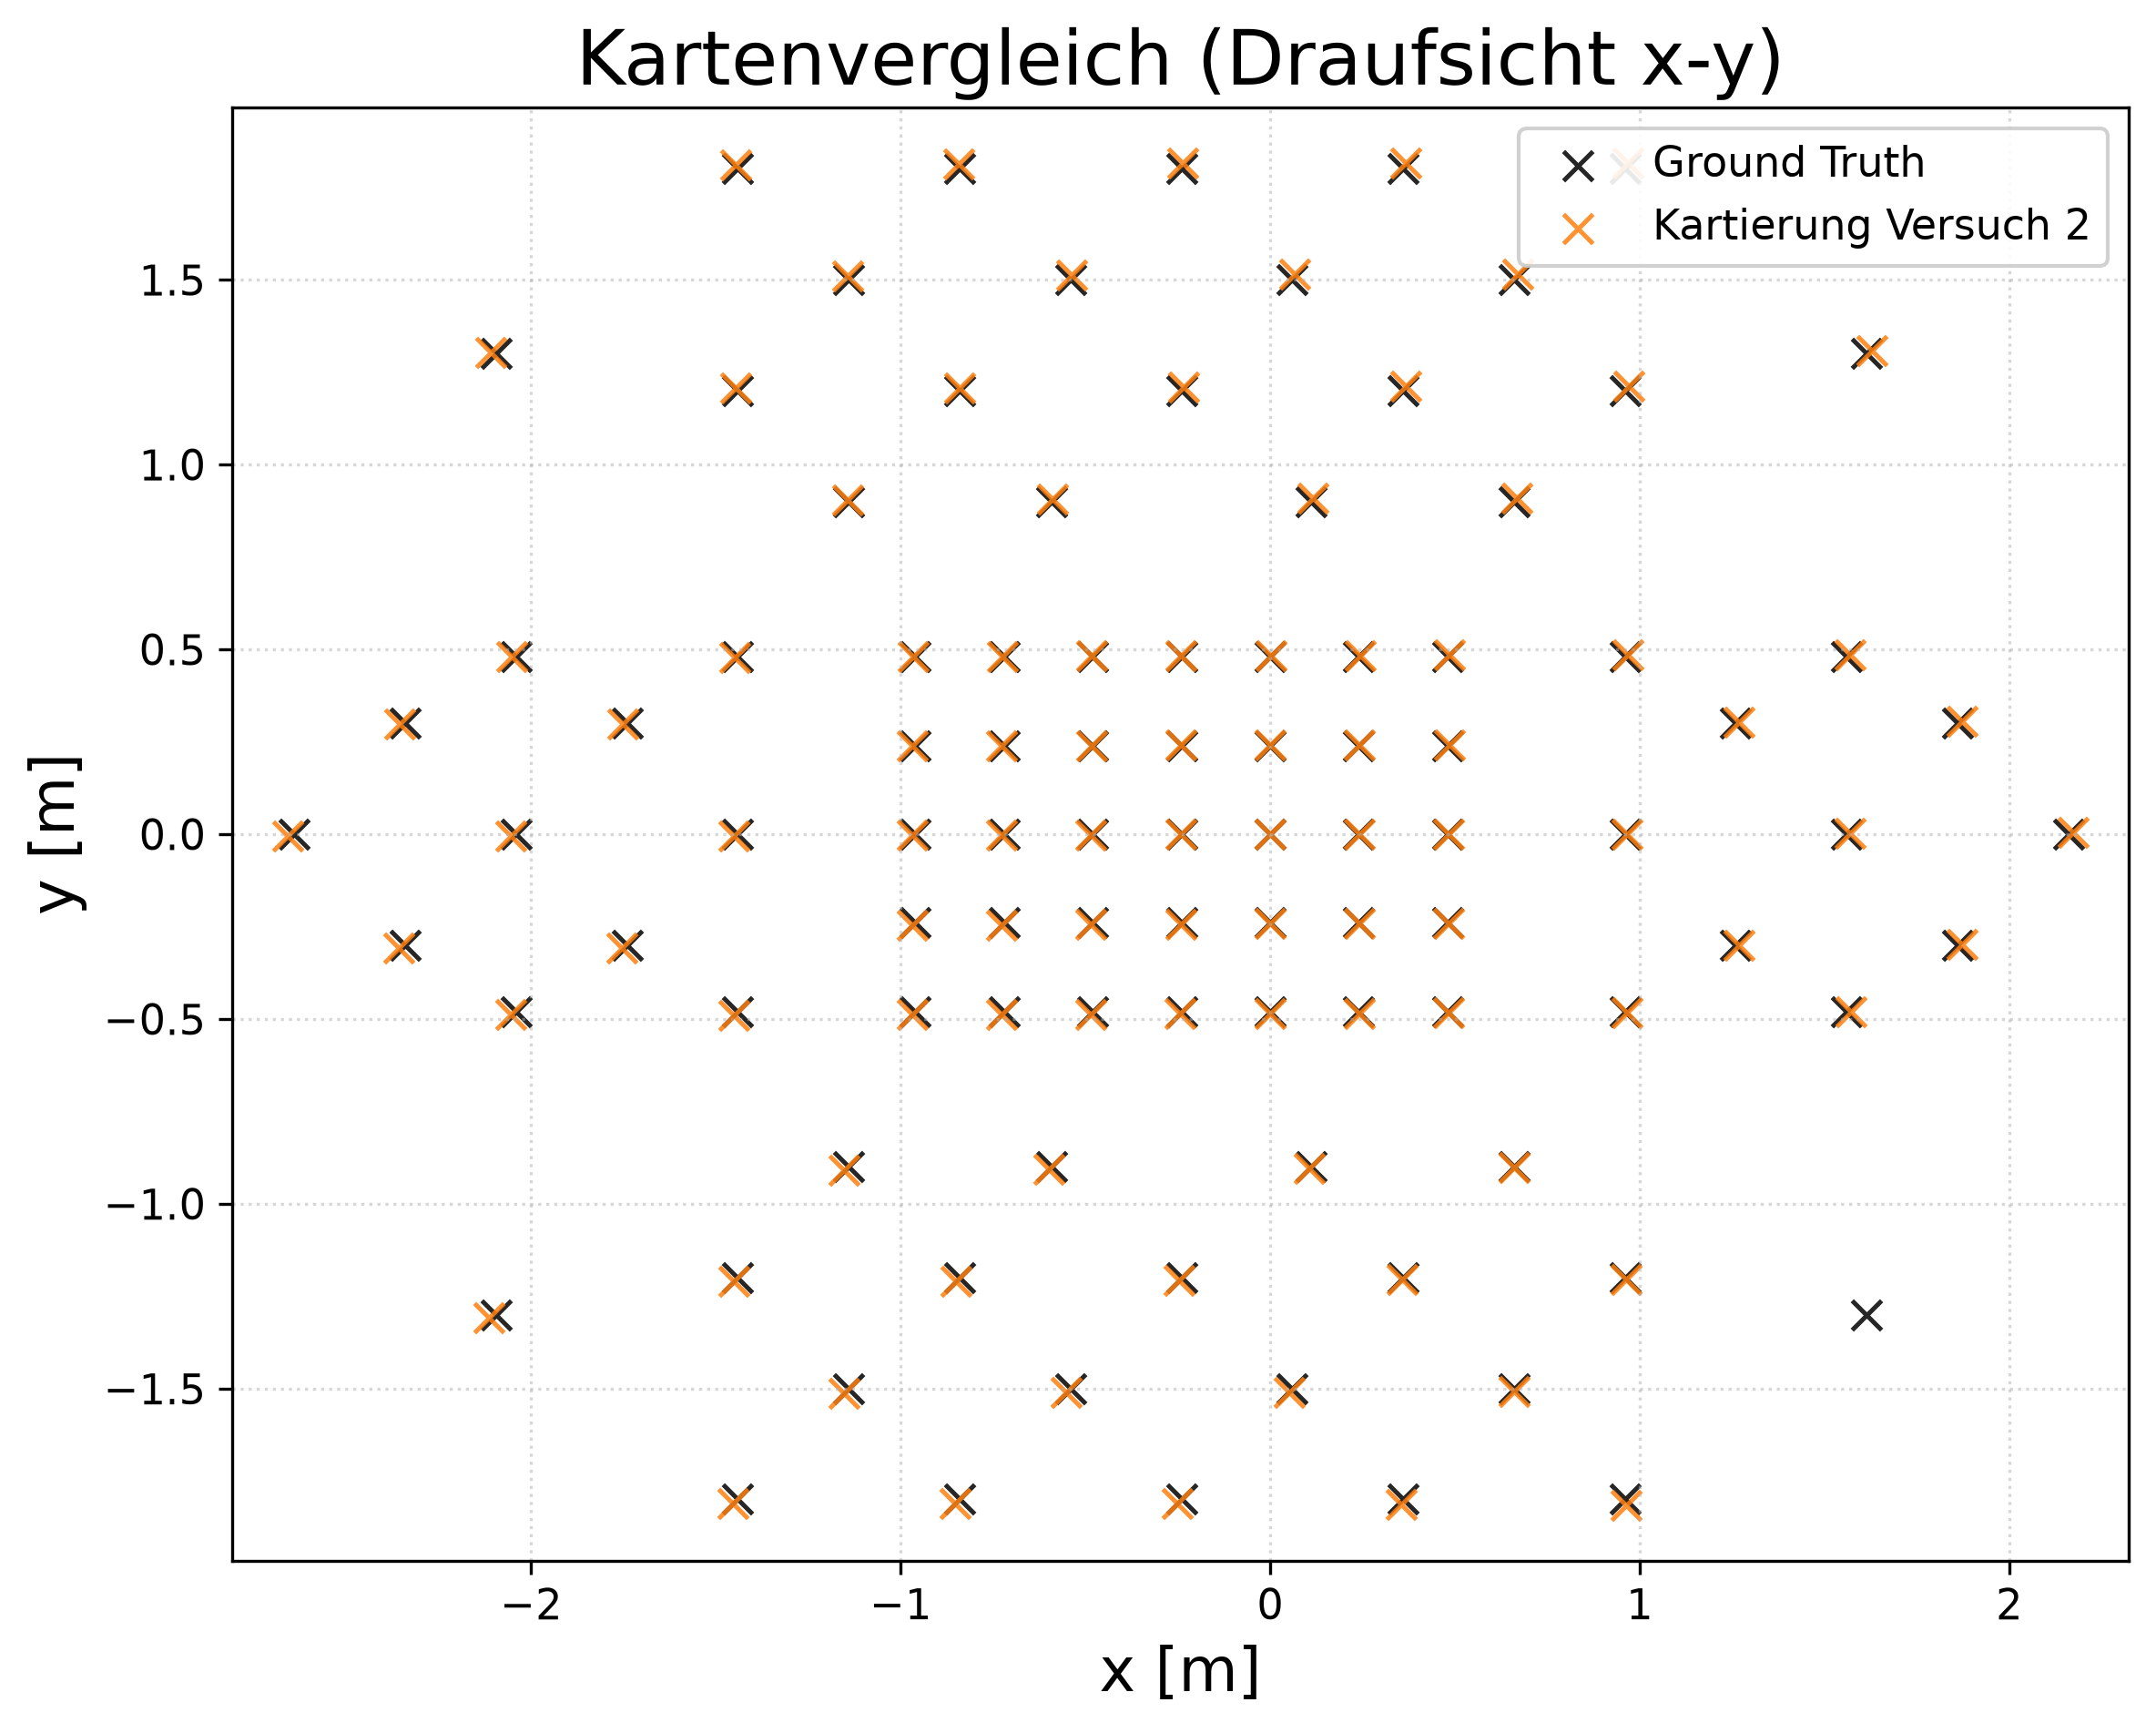
\includegraphics[width=0.7\textwidth]{Bilder/karten_vergleich_ueberlagert_Versuch_2.png}
    \caption{Überlagerung der in Versuch~2 erzeugten Karte mit der Ground Truth}
    \label{fig:kartenvergleich_versuch2}
\end{figure}
\FloatBarrier

\begin{figure}[htbp]
    \centering
    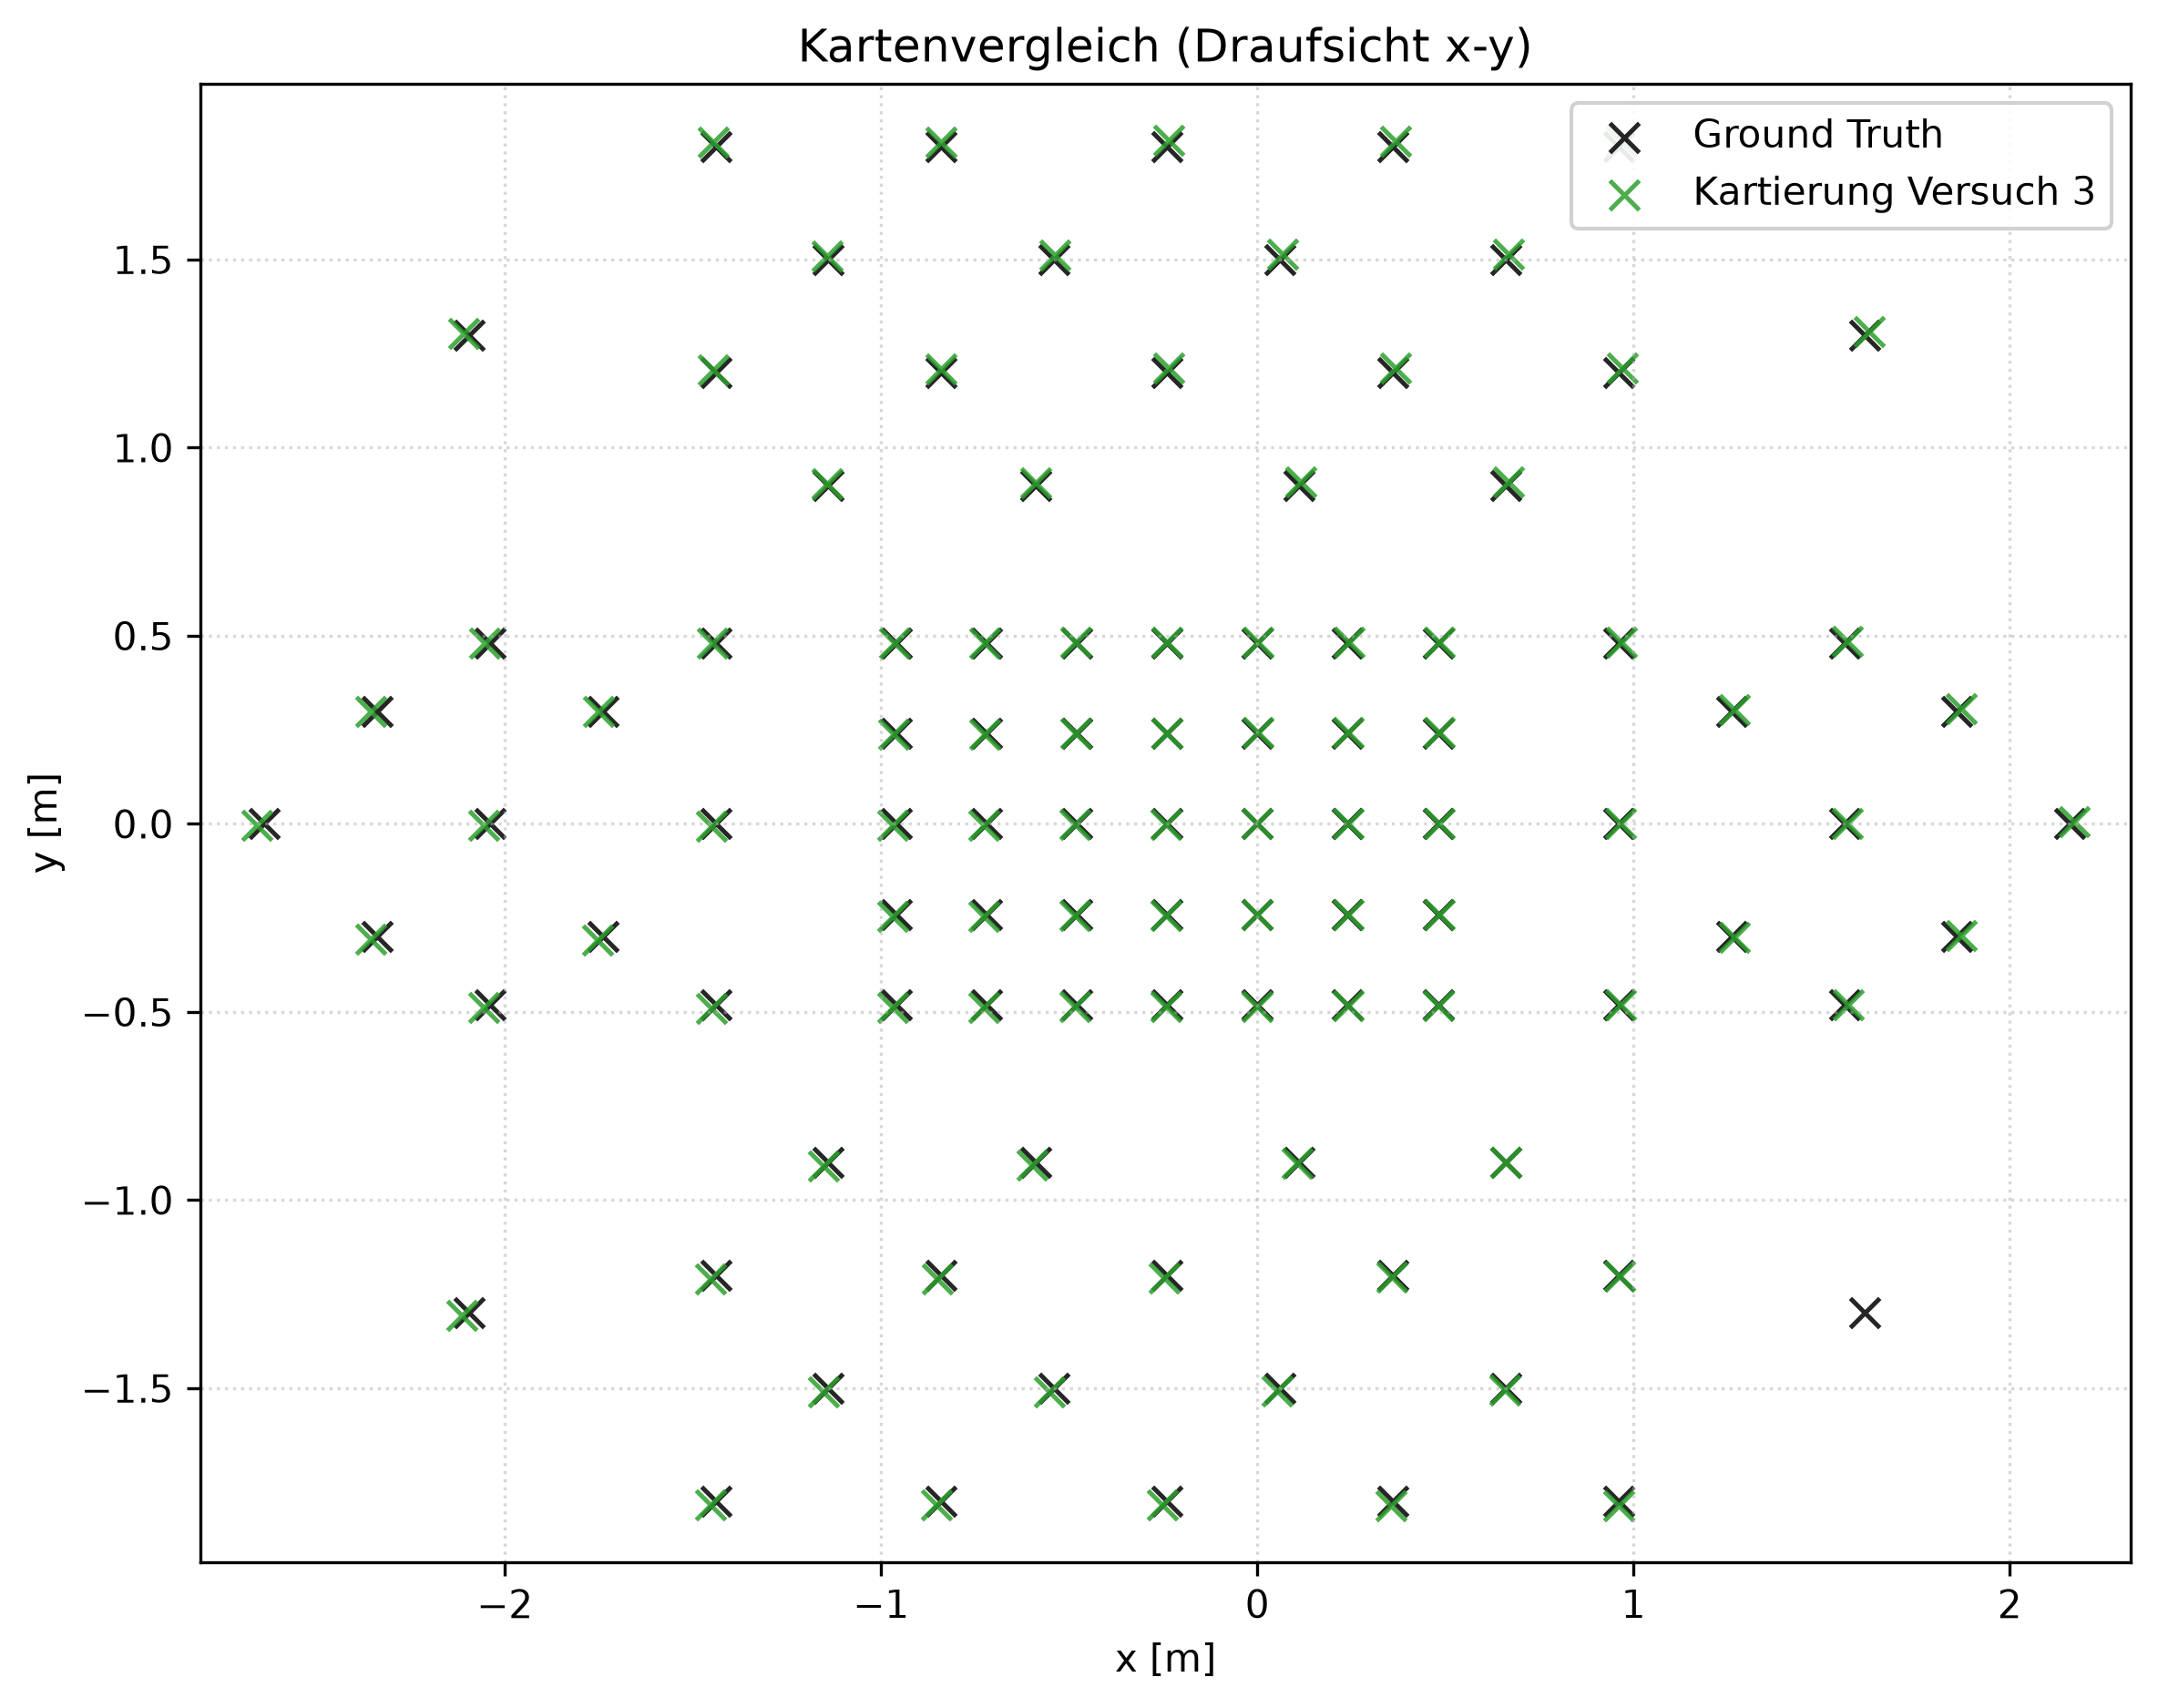
\includegraphics[width=0.7\textwidth]{Bilder/karten_vergleich_ueberlagert_versuch_3.png}
    \caption{Überlagerung der in Versuch~3 erzeugten Karte mit der Ground Truth}
    \label{fig:kartenvergleich_versuch3}
\end{figure}
\FloatBarrier

Die Abweichungen der drei erzeugten Karten gegenüber der Sollkarte sind in Tabelle~\ref{tab:karten_evaluation} zusammengefasst.
Als Kennzahlen dienen der Mittelwert der Beträge sowie die größte auftretende Einzelabweichung.
Beide werden achsweise für die Position, für den räumlichen euklidischen Abstand $d_{xyz}$ der Markerzentren sowie für die drei Orientierungswinkel ausgewiesen.
Ergänzend ist die Laufzeit der jeweiligen Optimierung aufgeführt.
\begin{table}[htbp]
\centering
\begin{tabular}{llccc}
\toprule
\textbf{Kennzahl} & \textbf{Einheit} & \textbf{Versuch~1} & \textbf{Versuch~2} & \textbf{Versuch~3} \\
\midrule
Gemeinsame Fiducial-Marker & --   & $96$ & $96$ & $96$ \\
Laufzeit          & h    & $0{,}75$ & $2$ & $9$ \\
\midrule
$\Delta x$ Mittelwert & mm & $8{,}33$ & $6{,}98$ & $6{,}87$ \\
$\Delta y$ Mittelwert & mm & $6{,}82$ & $6{,}10$ & $5{,}64$ \\
$\Delta z$ Mittelwert & mm & $4{,}74$ & $0{,}00$ & $0{,}00$ \\
\midrule
$\Delta x$ Maximum & mm & $24{,}58$ & $19{,}40$ & $20{,}74$ \\
$\Delta y$ Maximum & mm & $18{,}25$ & $16{,}66$ & $16{,}05$ \\
$\Delta z$ Maximum & mm & $19{,}11$ & $0{,}00$  & $0{,}00$ \\
\midrule
$d_{xyz}$ Mittelwert & mm & $12{,}75$ & $9{,}98$  & $9{,}57$ \\
$d_{xyz}$ Maximum    & mm & $32{,}27$ & $20{,}76$ & $21{,}75$ \\
\midrule
$\Delta\varphi_x$ Mittelwert & Grad & $0{,}33$ & $0{,}00$ & $0{,}00$ \\
$\Delta\theta_y$ Mittelwert  & Grad & $0{,}22$ & $0{,}00$ & $0{,}00$ \\
$\Delta\psi_z$ Mittelwert    & Grad & $0{,}10$ & $0{,}08$ & $0{,}08$ \\
\midrule
$\Delta\varphi_x$ Maximum & Grad & $1{,}29$ & $0{,}00$ & $0{,}00$ \\
$\Delta\theta_y$ Maximum  & Grad & $0{,}96$ & $0{,}00$ & $0{,}00$ \\
$\Delta\psi_z$ Maximum    & Grad & $0{,}42$ & $0{,}31$ & $0{,}34$ \\
\bottomrule
\end{tabular}
\caption[Abweichungen der erzeugten Karten gegenüber der Ground Truth Karte]{Abweichungen der erzeugten Karten gegenüber der Ground Truth Karte.}
\label{tab:karten_evaluation}
\end{table}
\FloatBarrier


Bereits die Karte aus Versuch~eins liegt nahe an der Ground Truth Karte.
Die Abweichung der Fiducial-Markerzentren beträgt im Mittel $8{,}33$~mm in $x$ und $6{,}82$~mm in $y$, im räumlichen Abstand $12{,}75$~mm.
Die Überlagerung in Abbildung~\ref{fig:kartenvergleich_versuch1} zeigt über die gesamte Fläche hinweg keine erkennbare systematische Verformung.
Erreicht wird dies bei einer Laufzeit von etwa $45$~min und ohne jedes Vorwissen über die Kartengeometrie.
Die Höhenabweichung von im Mittel $4{,}74$~mm und maximal $19{,}11$~mm ist dabei vollständig als Schätzfehler zu werten, da alle Fiducial-Marker flach auf dem Boden aufliegen.
Gleiches gilt für die Verkippungen von $0{,}33$~Grad in $\Delta\varphi_x$ und $0{,}22$~Grad in $\Delta\theta_y$.

Versuch~zwei senkt die Abweichung in der Kartenebene auf $6{,}98$~mm in $x$ und $6{,}10$~mm in $y$ und drückt die Höhe sowie die 
Verkippungen durch die Bindung an die Bodenebene auf null.
Der Rückgang des räumlichen Abstands auf $9{,}98$~mm geht damit nur zum Teil auf eine bessere Schätzung zurück, 
denn die $z$-Komponente entfällt dort als Fehlerquelle per Vorgabe.

Versuch~drei unterscheidet sich von Versuch~zwei im Betriebsmodus sowie der Häufigkeit der Optimierungen und liefert praktisch dasselbe Ergebnis.
Der mittlere räumliche Abstand sinkt um lediglich $0{,}41$~mm auf $9{,}57$~mm, während der Maximalwert von $20{,}76$~mm auf $21{,}75$~mm ansteigt.
In $\Delta\psi_z$, dem einzigen weiterhin geschätzten Winkel, liegen beide Läufe bei $0{,}08$~Grad.





Bei genauerer Betrachtung aller Karten fällt auf, dass mit steigendem Abstand zum Ursprung der Positionsfehler weiter ansteigt.
Abbildung~\ref{fig:dxyz_ueber_abstand} stellt dies anschaulich dar.
Für jeden Fiducial-Marker ist die euklidische Distanz zwischen seiner Position in der Kartierung und seiner Position in dem Ground Truth aufgetragen.
Diese Distanz ist über dem Abstand desselben Markers zum Ursprung dargestellt, der durch Tag~0 festgelegt ist.
Jeder Punkt entspricht damit einem Fiducial-Marker in einem der drei Läufe.
\newpage
\begin{figure}[htbp]
    \centering
    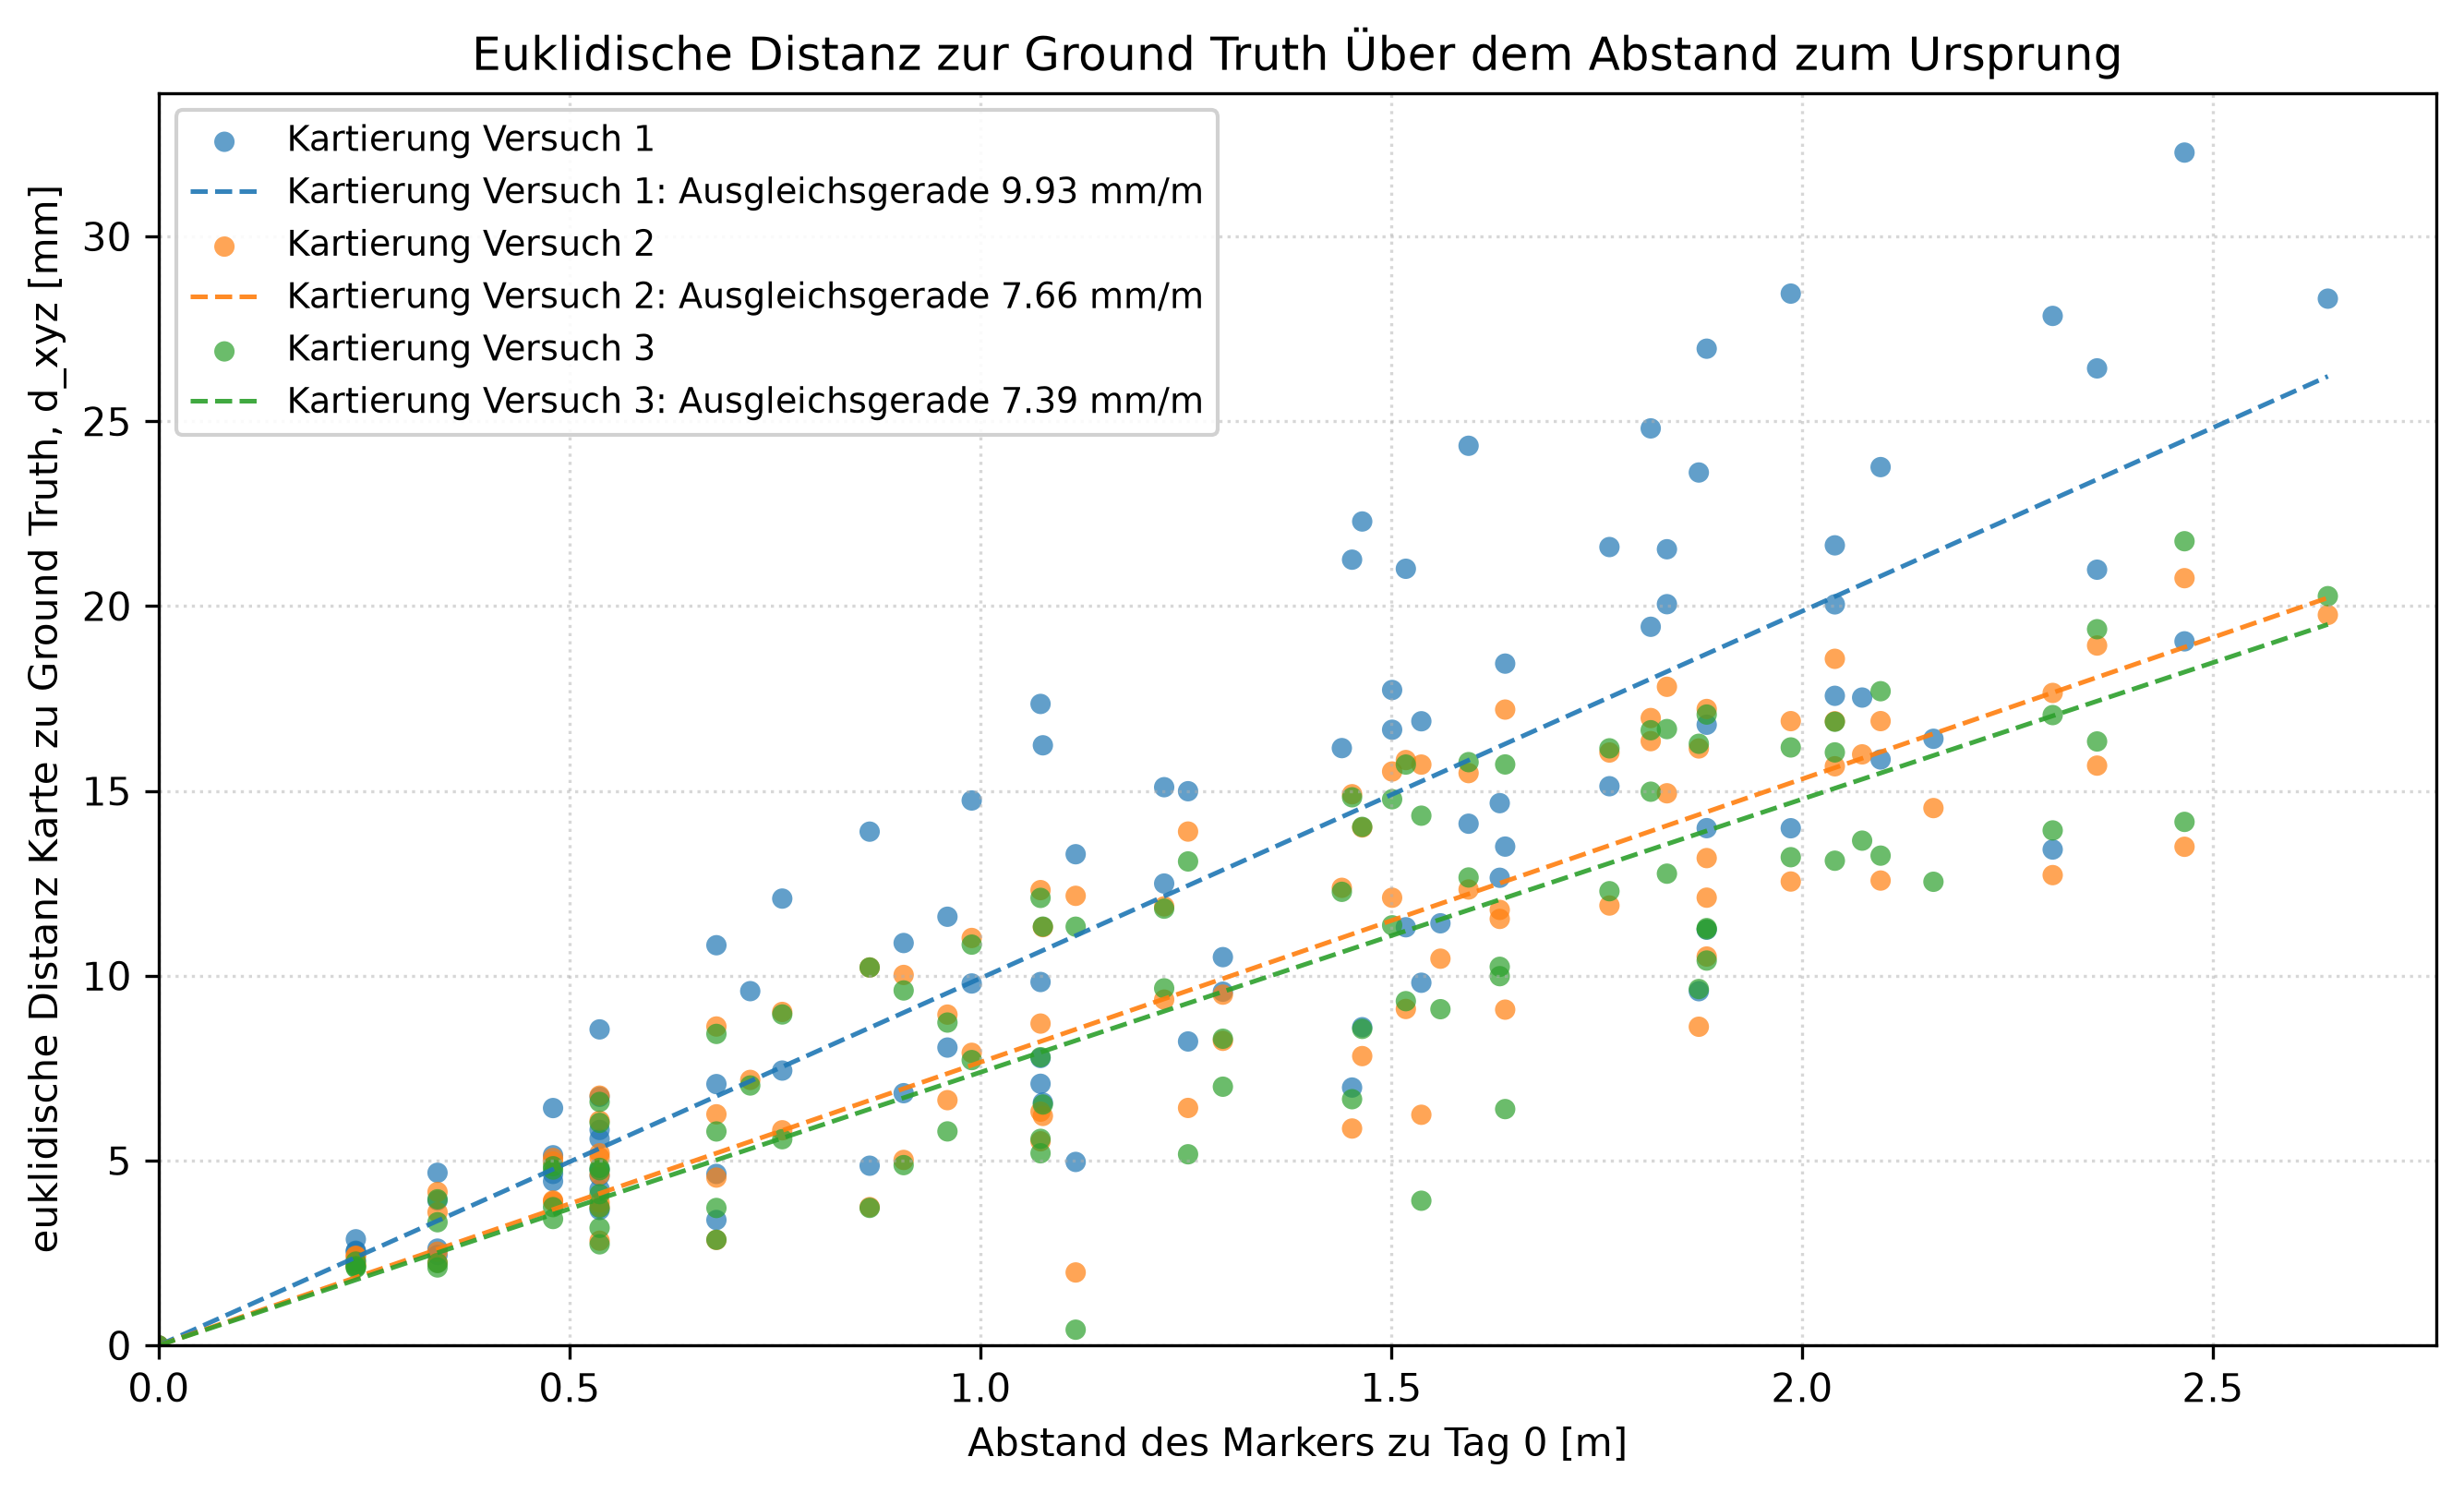
\includegraphics[width=1.0\textwidth]{Bilder/karten_vergleich_dxyz_ueber_tag0_punkte.png}
    \caption{Euklidische Distanz der Tag-Positionen zwischen Kartierung und Ground Truth in Abhängigkeit vom Abstand des jeweiligen Markers zum Ursprung.}
    \label{fig:dxyz_ueber_abstand}
\end{figure}


In der Nähe des Ursprungs liegen die Abweichungen aller drei Läufe bei wenigen Millimetern.
Am äußeren Rand des Kartierungsbereichs bei etwa 2,6~m Abstand erreichen sie dagegen Werte von bis zu rund 32~mm.
Der Anstieg verläuft dabei nicht sprunghaft, sondern über den gesamten Abstandsbereich gleichmäßig.

Zur Verdeutlichung dieses Zusammenhangs ist je Lauf eine Ausgleichsgerade durch den Ursprung eingezeichnet.
Ihre Steigung beschreibt den Zuwachs der Abweichung je Meter Abstand zum Ursprung.
Für den ersten Lauf beträgt sie 9,93~mm/m, für den zweiten Lauf 7,66~mm/m und für den dritten Lauf 7,39~mm/m.
Der zweite und der dritte Lauf liegen damit sehr nahe beieinander, während der erste Lauf über den gesamten Abstandsbereich die größten Abweichungen aufweist.

Bemerkenswert ist, dass alle drei Läufe demselben Verlauf folgen und sich lediglich in der Steigung unterscheiden.
Der Positionsfehler ist folglich kein konstanter Versatz der gesamten Karte, sondern wächst proportional zum Abstand vom Ursprung.


Alle drei Versuche liefern eine brauchbare Karte ohne grobe Fehler.
Der mittlere räumliche Abstand der Markerzentren zur Sollkarte liegt zwischen $9{,}57$~mm und $12{,}75$~mm, die größte Einzelabweichung zwischen $20{,}76$~mm und $32{,}27$~mm.
Von den 97 aufgebrachten Markern sind in jedem Versuch 96 in der Karte enthalten.
Die Unterschiede zwischen den Versuchen betreffen damit weniger die grundsätzliche Brauchbarkeit der Karte als vielmehr den Aufwand, mit dem sie erreicht wird.

Für die Kartierung einer neuen oder die Erweiterung einer bestehenden Umgebung empfiehlt sich das zweistufige Vorgehen aus Versuch~1 und Versuch~2.
Die Parametrierung des ersten Versuchs liefert innerhalb von etwa $45$~min eine Startschätzung, ohne dass Vorwissen über die Kartengeometrie erforderlich ist.
Deren Ergebnis geht anschließend als Startlage in die Parametrierung des zweiten Versuchs ein, der den mittleren räumlichen Abstand bei einer Laufzeit von etwa zwei Stunden senkt.

%Der Betriebsmodus \texttt{slow} aus Versuch~3 rechtfertigt den zusätzlichen Aufwand nicht.
%Gegenüber Versuch~2 sinkt der mittlere räumliche Abstand um lediglich $0{,}41$~mm, während der Maximalwert von $20{,}76$~mm auf $21{,}75$~mm ansteigt.
%Dem steht eine Laufzeit von neun Stunden gegenüber, also mehr als das Vierfache des zweiten Versuchs.
%Ein merklicher Gewinn an Genauigkeit ist damit nicht verbunden.
%
%Als wirksam erweist sich dagegen das Einbringen von Vorwissen in die Optimierung.
%Die Bindung aller Fiducial-Marker an die Bodenebene über $z=0$ sowie die auf null gesetzten Verkippungen um die $x$- und $y$-Achse entfernen drei Freiheitsgrade, die andernfalls als Schätzfehler in die Karte eingehen.
%In Versuch~1 äußert sich dies in einer Höhenabweichung von im Mittel $4{,}74$~mm sowie in Verkippungen von $0{,}33$~Grad im Rollen und $0{,}22$~Grad im Nicken, obwohl alle Fiducial-Marker flach auf dem Boden aufliegen.
%Bei der Aufzeichnung weiterer Karten sollte daher sämtliches verfügbare Wissen über die Geometrie der Umgebung in die Parametrierung einfließen.
%
%Die wesentliche verbleibende Fehlerquelle ist der in Abbildung~\ref{fig:dxyz_ueber_abstand} gezeigte Anstieg der Abweichung mit dem Abstand zum Ursprung.
%Da sich alle Fiducial-Marker allein anhand des Ursprungs optimieren, wächst die Abweichung je Meter Entfernung um $7{,}39$~mm bis $9{,}93$~mm.
%Um die Qualität der Karte nachhaltig zu verbessern, sollten daher, sofern möglich, etwa alle zwei bis drei Meter vermessene Referenzen vorgegeben werden.
%Solche zusätzlichen Stützstellen begrenzen die Strecke, über die sich der Fehler aufbauen kann und reduzieren damit den in Abbildung~\ref{fig:dxyz_ueber_abstand} erkennbaren Anstieg.






\section{Durchführung und Evaluation der Positionierung}
\label{sec:durchfuehrung_positionierung}
Dieser Abschnitt beschreibt den Ablauf der Flugversuche.
Dazu gehören die Bedienung des \gls{uav}s sowie die Wahl der Startparameter für den Flugbetrieb.
Im letzten Teil werden die Ergebnisse bewertet.

\subsection{Senden von Positions-Sollwerten an PX4}
\label{sec:bedienkonsole}
Zur Betrieb des \gls{uav}s während der Versuche kommen zwei Bedienwege zum Einsatz.
Die eigentliche Flugführung übernimmt der eigens entwickelte Node \texttt{control\_console\_uxrce}, der auf dem Begleitrechner ausgeführt wird.
Die Bedienung erfolgt über eine \gls{ssh}-Verbindung per W-LAN von dem externen Computer aus. 

Diese Bedienkonsole erfüllt zwei Aufgaben.
Zum einen nimmt sie Bedienbefehle entgegen und sendet daraufhin fortlaufend Positions-Sollwerte im Kartenkoordinatensystem an \gls{px4}.
Zum anderen führt sie den Zustand des Systems aus mehreren Quellen zusammen und zeigt ihn fortlaufend an.

Von \gls{px4} stammen der Fahrzeugstatus mit Verbindung, der Arm-Zustand, der Bedienmodus, die im \gls{ekf} geschätzte Position sowie die Bodenkontakterkennung.
Aus der Konsole selbst stammen die angesteuerte Zielposition und der jeweils aktive Sollwert-Modus.
Beide Positionsangaben werden in der \gls{enu}-Konvention der Karte ausgegeben.
Ergänzend prüft die Konsole die Verfügbarkeit der beiden Kameras.

Die Steuerung erfolgt vollständig über die Tastatur, deren Belegung Tabelle~\ref{tab:konsole_tasten} zusammenfasst.
\begin{table}[htbp]
\centering
\begin{tabular}{ll}
\toprule
\textbf{Taste} & \textbf{Funktion} \\
\midrule
\texttt{a}/\texttt{d}   & Sollwert in $x$ verschieben \\
\texttt{w}/\texttt{s}   & Sollwert in $y$ verschieben \\
\texttt{o}/\texttt{l}   & Sollwert in $z$ verschieben \\
\texttt{q}/\texttt{e}   & Gierwinkel-Sollwert verstellen \\
\texttt{Leertaste}      & Armieren, im armierten Zustand Landung an Ort und Stelle \\
\texttt{g}              & Demo-Modus starten, bei erneuter Betätigung abbrechen \\
\texttt{Esc}            & Konsole beenden \\
\bottomrule
\end{tabular}
\caption{Tastenbelegung der Bedienkonsole}
\label{tab:konsole_tasten}
\end{table}
\FloatBarrier

Über die Leertaste wird das \gls{uav} armiert.
Ist es bereits armiert, löst dieselbe Taste eine Landung an Ort und Stelle aus, 
bei der horizontale Position und Gierwinkel gehalten und die Höhe langsam abgesenkt werden, bis bei Bodenkontakt automatisch disarmiert wird.

Über die Taste \texttt{g} lässt sich ein autonomer Demo-Modus starten, in dem das \gls{uav} ein Quadrat abfliegt.
Es fliegt dazu mit konstanter Geschwindigkeit die nächstgelegene Ecke an, fliegt das Quadrat einmal ab und schwebt anschließend wieder an dieser Startecke.
Höhe und Gierwinkel bleiben während der gesamten Bewegung fest.
Erneutes Drücken von \texttt{g} bricht den Demo-Modus ab und hält die aktuelle Position.
Kantenlänge sowie Geschwindigkeit können über die Startparameter des Nodes eingestellt werden.

Sowohl die manuellen Sollwertänderungen als auch die Bewegung im Demo-Modus sind in ihrer Geschwindigkeit begrenzt.
Translatorisch gilt eine Begrenzung auf $1{,}5$~m/s in der $x$-$y$-Ebene und auf $3{,}0$~m/s in $z$.
Eine besondere Rolle spielt dabei die Giergeschwindigkeit.
Ein Multicopter giert, indem er das Reaktionsmoment der Rotoren gezielt verstimmt, wozu ein Teil der Motoren beschleunigt und der andere verlangsamt wird.
Je schneller gegiert werden soll, desto größer fällt diese Drehzahldifferenz aus und desto höher steigt die geforderte Drehzahl der beschleunigenden Motoren.
Ein schneller Gierbefehl treibt sie dann in die Sättigung, sodass sie das für das Giermoment und den Auftrieb gleichzeitig benötigte Drehmoment nicht mehr aufbringen können.
Der Gesamtschub sackt in der Folge ab und die Flughöhe kann während des Gierens nicht mehr gehalten werden.
Die maximale Giergeschwindigkeit wird daher bewusst niedrig auf maximal $20^\circ$/s gewählt.

Ergänzend zum Control-Node wird die Fernsteuerung zum Umschalten der Flugmodi und zum Eingriff bei Fehlfunktionen genutzt.
Über sie wird der \texttt{Offboard} Modus als regulärer Betriebsmodus aktiviert, in dem die Konsole die Sollwerte vorgibt.
Für den Störfall sind zwei weitere Schalter vorgesehen.
Der erste wechselt in den Modus \texttt{Auto.Land}, in dem das \gls{uav} selbstständig und gezielt landet.
Der zweite stoppt als Notausschalter die Rotoren unmittelbar und dient als letzte Sicherungsmaßnahme. 
Ergänzend ist der \gls{px4} so konfiguriert, dass das \gls{uav} automatisch landet, sobald die Verbindung zur Fernsteuerung oder zum Node verloren geht.

\subsection{Wahl der Startparameter für den Flugbetrieb}
\label{subsec:pos_parametrierung}
Die Startparameter des Nodes \texttt{vision\_pose\_uxrce\_node} wurden auf den geplanten Flugbetrieb abgestimmt.
Ausschlaggebend sind eine nominelle Flughöhe von etwa 1,8~m, eine senkrecht nach unten gerichtete Kamera und eine Karte mit unterschiedliche großen Markern.

Die Karte liegt im vorliegenden Aufbau ausschließlich am Boden, sodass die Frontkamera keine Fiducial-Marker erfassen kann.
Sie ist deshalb über \texttt{cam2\_weight}${}=0$ aus der Fusion ausgeschlossen.
Die konkret gewählten Werte sind in Tabelle~\ref{tab:vision_pose_werte} zusammengefasst, die Bedeutung der einzelnen Parameter sind in Tabelle~\ref{tab:vision_pose_params} erläutert.

{\footnotesize
\begin{longtable}{@{}l r@{}}
\toprule
\textbf{Parameter} & \textbf{Wert} \\
\midrule
\endfirsthead

\multicolumn{2}{@{}l}{\footnotesize\itshape Fortsetzung von Tabelle~\ref{tab:vision_pose_werte}} \\
\toprule
\textbf{Parameter} & \textbf{Wert} \\
\midrule
\endhead

\midrule
\multicolumn{2}{r@{}}{\footnotesize\itshape Fortsetzung auf der nächsten Seite} \\
\endfoot

\bottomrule
\caption{Für den Flugbetrieb gewählte Startwerte des Nodes \texttt{vision\_pose\_uxrce\_node}}
\label{tab:vision_pose_werte}
\endlastfoot

\multicolumn{2}{@{}l}{\textit{Karte und Kalibrierung}} \\
\texttt{map\_file}                         & Pfad \\
\texttt{calibration\_file}                 & Pfad \\
\addlinespace
\multicolumn{2}{@{}l}{\textit{Topics und Bezugssysteme}} \\
\texttt{cam1\_topic}                       & \texttt{/camera\_1/tag\_detections} \\
\texttt{cam1\_name}                        & \texttt{camera\_1} \\
\texttt{publish\_topic}                    & \texttt{/fmu/in/vehicle\_visual\_odometry} \\
\texttt{map\_frame}                        & \texttt{tag\_map} \\
\addlinespace
\multicolumn{2}{@{}l}{\textit{PX4-Anbindung und Zeit}} \\
\texttt{pose\_frame}                       & $1$ \\
\texttt{timesync\_topic}                   & \texttt{/fmu/out/timesync\_status} \\
\addlinespace
\multicolumn{2}{@{}l}{\textit{Ausreißerfilterung (RANSAC)}} \\
\texttt{ransac\_base\_threshold\_m}        & $0{,}06$ \\
\texttt{ransac\_reference\_distance\_m}    & $1{,}4$ \\
\texttt{ransac\_min\_inliers\_ratio}       & $0{,}70$ \\
\texttt{ransac\_max\_iterations}           & $10$ \\
\texttt{ransac\_max\_distance\_factor}     & $4{,}0$ \\
\addlinespace
\multicolumn{2}{@{}l}{\textit{Fusion und Glättung}} \\
\texttt{publish\_rate\_hz}                 & $50$ \\
\texttt{max\_estimate\_age\_s}             & $0{,}03$ \\
\texttt{cam1\_weight}                      & $1{,}0$ \\
\texttt{cam2\_weight}                      & $0{,}0$ \\
\texttt{position\_smoothing\_alpha}        & $0{,}3$ \\
\texttt{rotation\_smoothing\_alpha}        & $0{,}3$ \\
\texttt{min\_tags\_required}               & $1$ \\
\addlinespace
\end{longtable}
}

Die Bodenkamera wird mit einer Auflösung von 1280~$\times$~720 und 60~\gls{fps} betrieben.
Die Ausgaberate liegt mit \texttt{publish\_rate\_hz}${}=50$~Hz bewusst darunter.
Damit bleibt die geforderte untere Grenze von 30~\gls{fps} aus Abschnitt~\ref{sec:pos_ekf_konfiguration} deutlich überschritten, während die Reserve zur Bildrate dafür sorgt, dass der Takt auch dann eingehalten wird, 
wenn einzelne Bilder verzögert eintreffen oder ausfallen.

Der Parameter \texttt{max\_estimate\_age\_s}${}=0{,}03$~s ist auf diesen Bildtakt abgestimmt.
Der Ausfall eines einzelnen Bildes wird damit toleriert, während bei längerem Ausfall keine veraltete Schätzung mehr ausgegeben wird und der \gls{ekf} die Lücke über \gls{drl} überbrückt.
Der Parameter \texttt{min\_tags\_required}${}=1$ erlaubt die Positionsbestimmung bereits mit einem einzigen sichtbaren Marker.
Beim Start liegt lediglich der Startmarker im Sichtfeld, sodass eine höhere Mindestanzahl die Lokalisierung in dieser Phase verhindern würde.

Die Schwelle der Ausreißerfilterung nach Gleichung~\eqref{eq:pos_ransac_schwelle} ergibt sich aus zwei Vorgaben.
Die Basisschwelle beträgt \texttt{ransac\_base\_threshold\_m}${}=0{,}06$~m, der zugehörige Bezugsabstand \texttt{ransac\_reference\_distance\_m}${}=1{,}4$~m.
Der Bezugsabstand wurde iterativ bestimmt, da bei einem höheren Wert zu viele Detektionen verworfen wurden.


Die obere Schranke $f_{\max}$ aus Gleichung~\eqref{eq:pos_ransac_schwelle} wird über \texttt{ransac\_max\_distance\_factor}${}=4{,}0$ vorgegeben und begrenzt den Schwellenwert auf $0{,}24$~m.
Die untere Schranke begrenzt den Schwellenwert bei Abständen unterhalb von rund $1{,}06$~m auf $0{,}05$~m.

Der Parameter \texttt{ransac\_max\_iterations}${}=10$ begrenzt die Zahl der Hypothesen.
Über \texttt{ransac\_min\_inliers\_ratio}${}=0{,}70$ wird nach Gleichung~\eqref{eq:pos_ransac_konsens} gefordert, dass mindestens $70$~Prozent aller Schätzungen der Konsensmenge angehören.

Die Glättungsfaktoren \texttt{position\_smoothing\_alpha} und \texttt{rotation\_smoothing\_alpha} wurden mit jeweils $0{,}3$ iterativ bestimmt.
Sie dämpfen nach den Gleichungen~\eqref{eq:pos_ema} und~\eqref{eq:pos_slerp} das Rauschen der einzelnen Detektionen, ohne die Schätzung übermäßig träge werden zu lassen.

Der Parameter \texttt{isaac\_reference\_size}${}=0{,}170$~m entspricht der Markergröße, mit der die Detektion im Container konfiguriert ist.
Da dort nur eine einzige Größe hinterlegt werden kann, die Karte aber vier verschiedene Kantenlängen enthält, korrigiert der Node die Translation abweichend großer Fiducial-Marker über das Verhältnis zur hinterlegten Bezugsgröße.



\subsection{Ablauf der Flugversuche}
\label{subsec:ablauf_flugversuche}
Im Vorhinein wurden Testflüge mit dem Ground Truth und den Versuchskarten 1 bis 3 durchgeführt, ohne einen merklichen Unterschied in der Positioniergenauigkeit festzustellen.
Bei den aufgezeichneten Karten wurde jeweils der Fiducial-Marker mit der \gls{id}~202 händisch eingetragen.
Die eigentliche Versuchsdurchführung fand mit der Ground Truth statt. 

Bevor die Flugversuche durchgeführt werden, wird die extrinsische Kalibrierung der Kamera nach Abschnitt\ref{subsec:extrinsische_kalibrierung_2} durchgeführt.
Sie liefert die Transformation von der Kamera zum Drohnenmittelpunkt, die nach Gleichung~\eqref{eq:pos_drohne} unmittelbar in die Positionsbestimmung eingeht.
Anschließend werden die Nodes der Verarbeitungskette mit der zuvor beschriebenen Parametern gestartet.

Sämtliche Versuche finden bei eingeschalteter Hallenbeleuchtung statt, wodurch die Lichtverhältnisse über alle Flüge hinweg konstant bleiben.

Die Versuche folgen einem festen Ablauf.
Das \gls{uav} steht zu Beginn über dem Startmarker im geometrischen Zentrum der Karte.
Über die Leertaste wird es armiert und steigt auf die Flughöhe von 1,8~m.
Dort verharrt es kurz über dem Kartenmittelpunkt, sodass sich die Zustandsschätzung einschwingen kann.
Anschließend wird über die Taste \texttt{g} der Demo-Modus aktiviert, in dem das \gls{uav} ein Quadrat mit einer Kantenlänge von 2~m abfliegt und danach an der Startecke schwebt.
Zum Abschluss löst die Leertaste die Landung an Ort und Stelle aus, bei der das \gls{uav} bei Bodenkontakt automatisch disarmiert.
Abbildung~\ref{fig:uav_im_flug} zeigt das \gls{uav} während dieses Manövers über der Karte.

\begin{figure}[htbp]
    \centering
    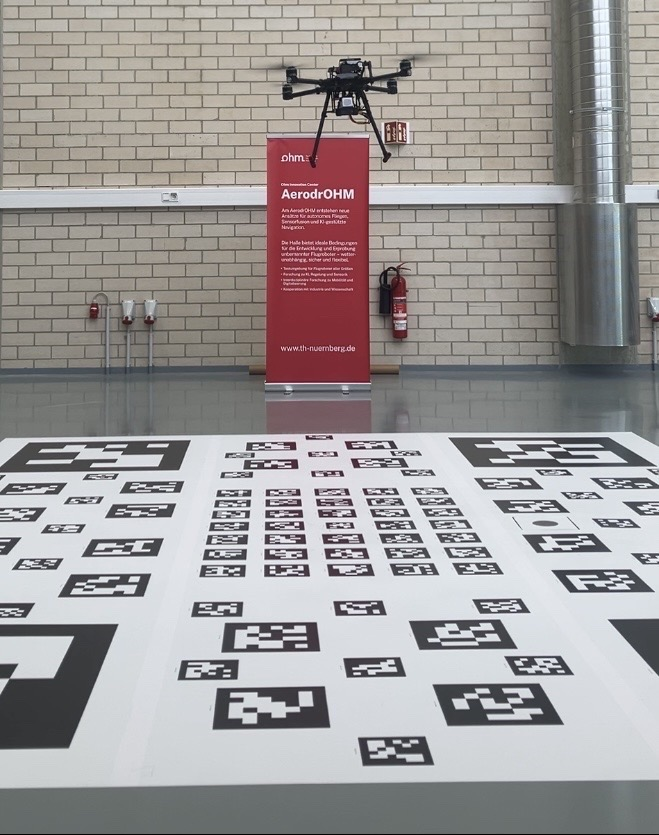
\includegraphics[width=0.50\textwidth]{Bilder/Drohne_schwebeflug.jpeg}
    \caption{Das \gls{uav} im Schwebeflug über der Markerkarte der OIC-Flughalle.}
    \label{fig:uav_im_flug}
\end{figure}
\FloatBarrier

Ein Versuch gilt als erfolgreich, wenn das \gls{uav} den beschriebenen Ablauf vollständig durchläuft.
Maßgeblich ist damit allein, ob das Manöver ohne Eingriff über die Fernsteuerung und ohne Abbruch zu Ende geführt wird.
Dieses Kriterium bewertet das Zusammenspiel der gesamten Verarbeitungskette, nicht die Genauigkeit der einzelnen Schätzung.




\subsection{Evaluation der Positionierung}
\label{subsec:evaluation_positionierung}
Insgesamt wurden drei Testflüge nach dem zuvor beschriebenen Schema durchgeführt.
Alle drei Flüge durchliefen den Ablauf vollständig und gelten damit als erfolgreich.
Da sich die Flüge im Ergebnis nicht unterscheiden, erfolgt die Auswertung beispielhaft an einem von ihnen.

Als Datengrundlage dient die Protokolldatei des Flugcontrollers.
Zwischen den Flügen treten geringfügige Unterschiede in den Protokollen auf, die das grundsätzliche Verhalten des Systems jedoch unberührt lassen.

Der Flug umfasst 77,1~s, wovon sich das \gls{uav} von 1,9~s bis 74,9~s in der Luft befindet.
Der Steigflug führt auf die Sollhöhe von 1,8~m, der Demo-Modus beginnt bei 23,0~s und fliegt ein Quadrat mit einer Kantenlänge von 2,0~m, bevor der Sinkflug bei 64,6~s einsetzt.
Über 97,1~Prozent der Zeit steht das \gls{uav} im Modus \texttt{Offboard}, den es erst zur Landung verlässt.

Abbildung~\ref{fig:Flugbahn} zeigt die vom Flugcontroller berechnete Flugbahn des \gls{uav}s.
Armierung und Landung sind jeweils farbig markiert. 
\begin{figure}[htbp]
    \centering
    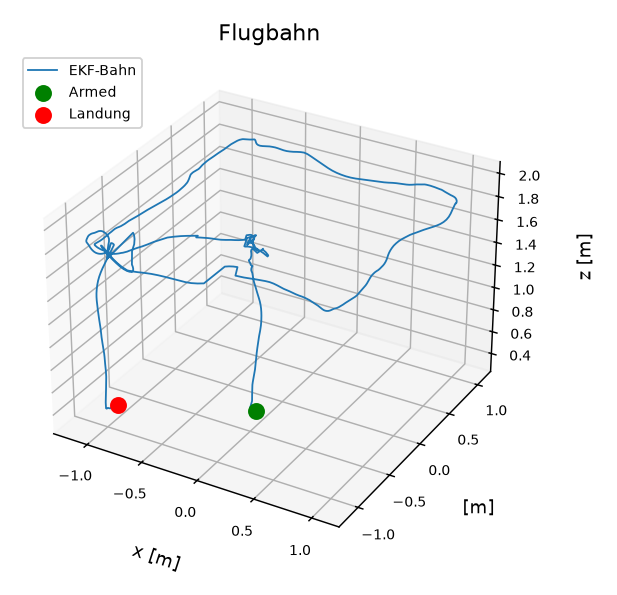
\includegraphics[width=0.6\textwidth]{Bilder/Flugbahn_testversuch.png}
    \caption{Berechnete Flugbahn des Flugcontrollers.}
    \label{fig:Flugbahn}
\end{figure}
\FloatBarrier


An dieser Stelle ist die Reichweite der Auswertung zu benennen.
Der Flugcontroller verfügt über keine unabhängige Referenz der wahren Pose, weshalb sich die absolute Genauigkeit der Positionsbestimmung aus dem Protokoll nicht bestimmen lässt.
Bewertbar ist stattdessen die Konsistenz der Fusion, also die Frage, ob die eingespeiste Position und die aus der \gls{imu} fortgeschriebene Vorhersage zueinander passen.

\subsection*{Belegung der Bezugsquellen des Zustandsschätzers}
Abbildung~\ref{fig:stuetzquellen} zeigt, welche Bezugsquellen der im Flugcontroller implementierte \gls{ekf} über den Flug hinweg zur Positionsschätzung heranzieht.

\begin{figure}[htbp]
\centering
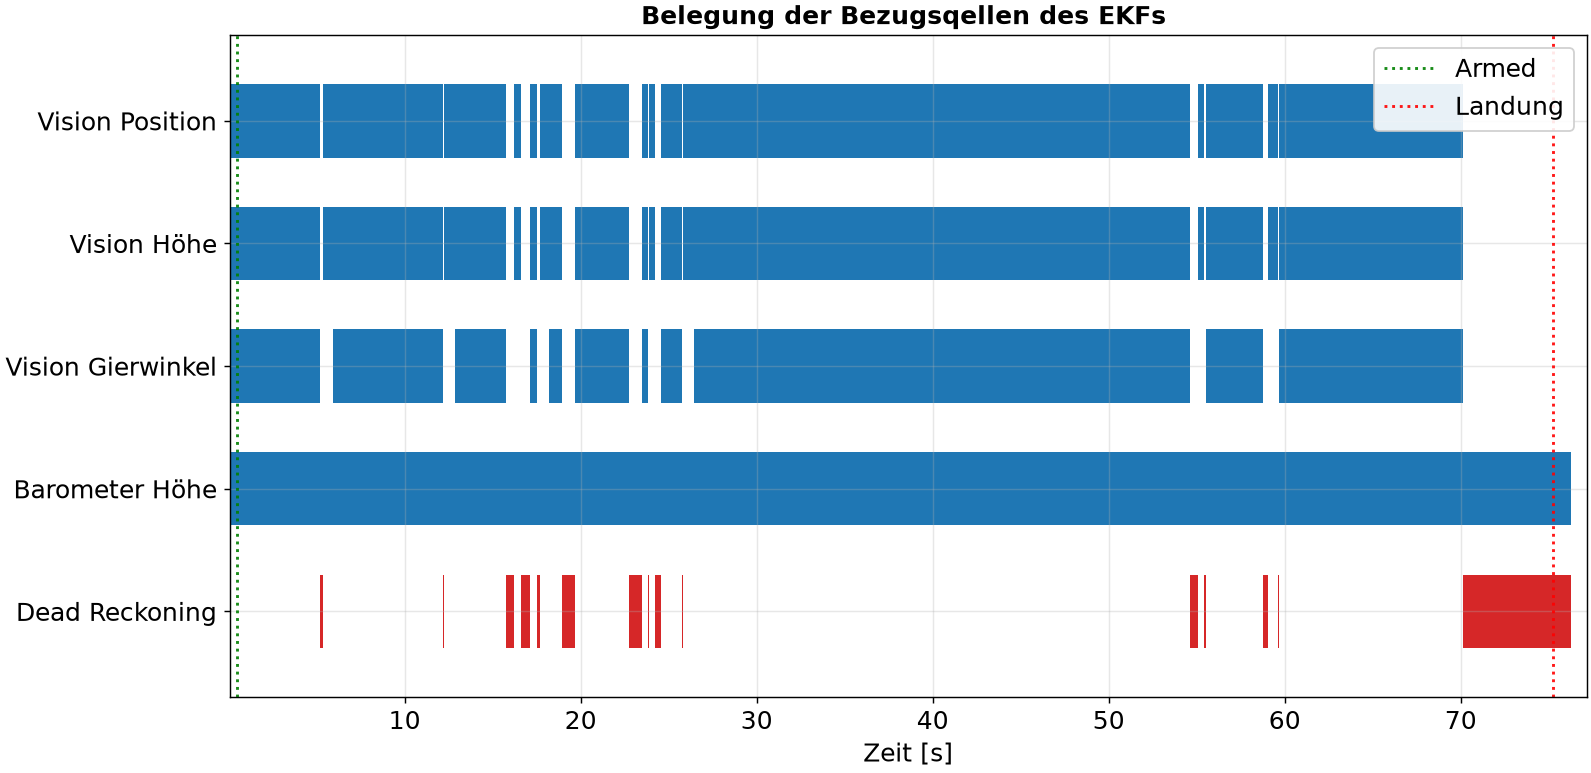
\includegraphics[width=1.0\textwidth]{Bilder/16_stuetzquellen.png}
\caption{Zeitliche Belegung der Stützquelen des \gls{ekf}s}
\label{fig:stuetzquellen}
\end{figure}
\FloatBarrier

Die Eingänge für Position, Höhe und Gierwinkel der Vision stammen aus der implementierten Positionsbestimmung.
Alle drei Flüge weisen während der Flugzeit kurze Aussetzer auf, deren längster 0,75~s dauert.
Bei der Landung unterschreitet das \gls{uav} diejenige Höhe, ab der die Kamera keinen Fiducial-Marker mehr vollständig erfasst, 
sodass die Positionsbestimmung ab 70,1~s bis zum Aufsetzen ausfällt.

Die Ursache über das Fehlen der Positionswerte kann aus den Protokolldateien nicht abgeleiet werden.
Während der Aussetzuer wurden von dem Node zur Positionsbestimmung keine Daten gesendet.
Mögliche Ursachen sind, keine Fiducial-Marker im Bild oder schlechte Markerdetektionen, sodass der Positionierungskonoten keine Daten ausgibt.

Während dieser Phasen wechselt der Zustandsschätzer auf \gls{drl} und schreibt die Position allein aus den Messungen der \gls{imu} fort.
Sämtliche Aussetzer bleiben deutlich unterhalb der Grenze von 5~s, die über \texttt{EKF2\_NOAID\_TOUT} eingestellt ist.
Die gestützte Navigation wird daher zu keinem Zeitpunkt verlassen.

Das intern verbaute Barometer ist über den gesamten Flug aktiv und liefert konstant Messwerte zur Flughöhe.



\newpage

\subsection*{Kalman-Gain der Vision-Positionsstützung}
\label{subsec:kalman_gain}
\begin{figure}[htbp]
\centering
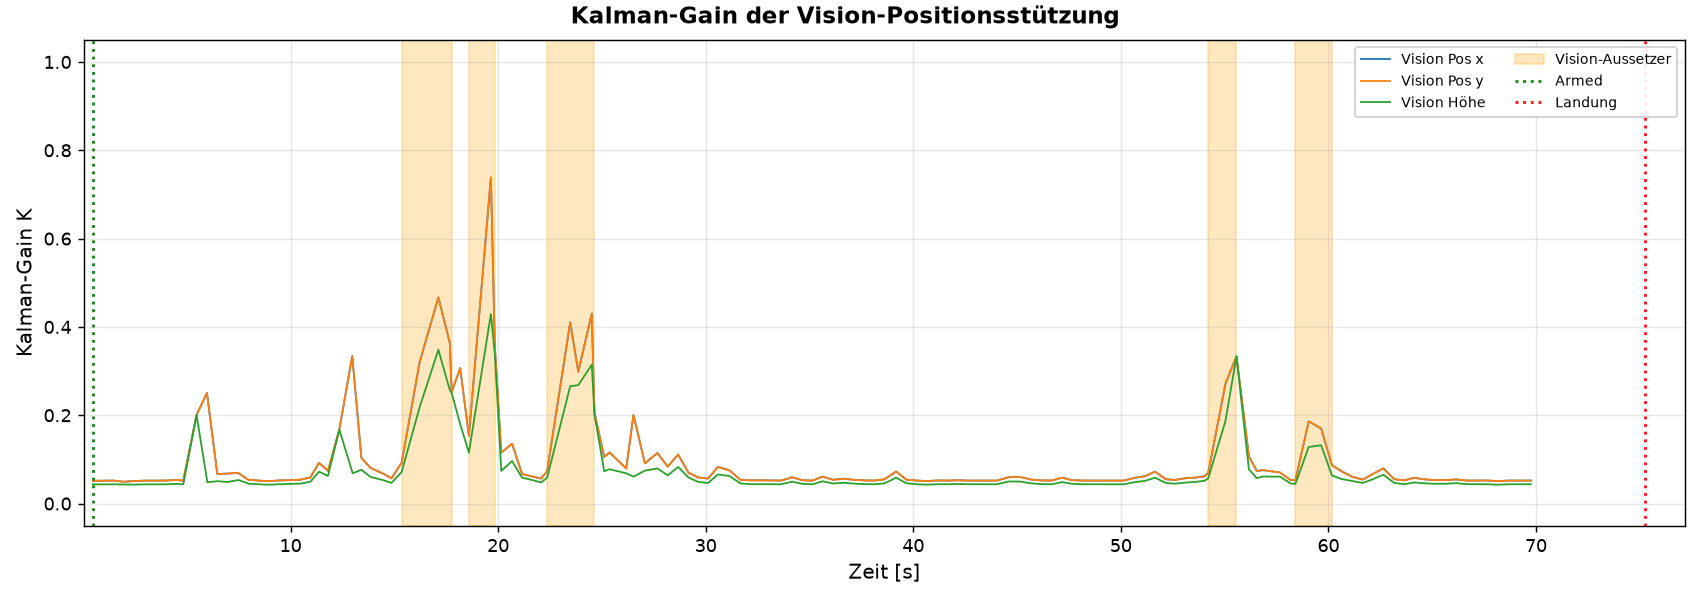
\includegraphics[width=1.0\textwidth]{Bilder/Kalman_Gain.png}
\caption{Verlauf des gespeicherten Kalman-Gains der Vision-Stützung.}
\label{fig:kalman_gain}
\end{figure}
\FloatBarrier

Abbildung~\ref{fig:kalman_gain} zeigt den Zeitlichen Verlauf des Klman-Gains während des Testflugs.
Über weite Teile des Fluges verläuft der Kalman-Gain auf einem konstanten, niedrigen Niveau.
Der Filter befindet sich dort im eingeschwungenen Zustand, in dem jedes Update genau so viel Unsicherheit abbaut, wie seit der letzten Korrektur durch das Prozessrauschen $\mathbf{Q}$ hinzugekommen ist.
Die Zustandskovarianz $\mathbf{P}$ bleibt dadurch klein und stabil.

Die Spitzen im Verlauf fallen mit den Unterbrechungen der Vision-Stützung zusammen.
In diesen Abschnitten entfällt die Korrekturphase und der Filter schreibt seinen Zustand allein über das Systemmodell fort.
Die Zustandskovarianz wächst dabei ausschließlich durch das Prozessrauschen an, während die Messrauschkovarianz $\mathbf{R}$ unverändert bleibt.
Das Verhältnis der beiden Unsicherheiten verschiebt sich zugunsten der Messung, sodass der Filter der eigenen Prädiktion weniger und den wieder einsetzenden Vision-Messungen entsprechend stärker vertraut.

Das im eingeschwungenen Zustand niedrige Niveau des Kalman-Gains ergibt sich aus dem Verhältnis von Prozessrauschen und Messrauschen.
Der Parameter \texttt{EKF2\_EVP\_NOISE} gibt für die Vision-Position eine Standardabweichung von \SI{0.1}{\meter} vor, die der Filter wegen \texttt{EKF2\_EV\_NOISE\_MD}~$=1$ für jede Messung ansetzt.
Da die Prädiktion zwischen zwei Vision-Messungen deutlich weniger stark abweicht als die angenommene Messunsicherheit, gewichtet der Filter die Modellvorhersage entsprechend höher.
Eine einzelne Vision-Messung geht damit nur zu einem geringen Anteil in die Zustandsschätzung ein, wirkt jedoch über eine Vielzahl aufeinanderfolgender Korrekturschritte.

Für weiterführende Arbeiten bietet sich an, die tatsächliche Streuung der Vision-Lokalisierung zu bestimmen und die Annahme für $\mathbf{R}$ daran auszurichten.
Fällt die tatsächliche Streuung geringer aus als die angenommenen \SI{0.1}{\meter}, kann der Parameter abgesenkt oder über \texttt{EKF2\_EV\_NOISE\_MD\,=0}~ durch eine pro Nachricht berechnete Kovarianz ersetzt werden.
Die Vision-Messungen würden dann stärker gewichtet und die Positionsunsicherheit des Filters weiter sinken.





\newpage

\subsection*{Verlauf der Positionsschätzung}
\label{subsec:positionsschätzung}
\begin{figure}[htbp]
\centering
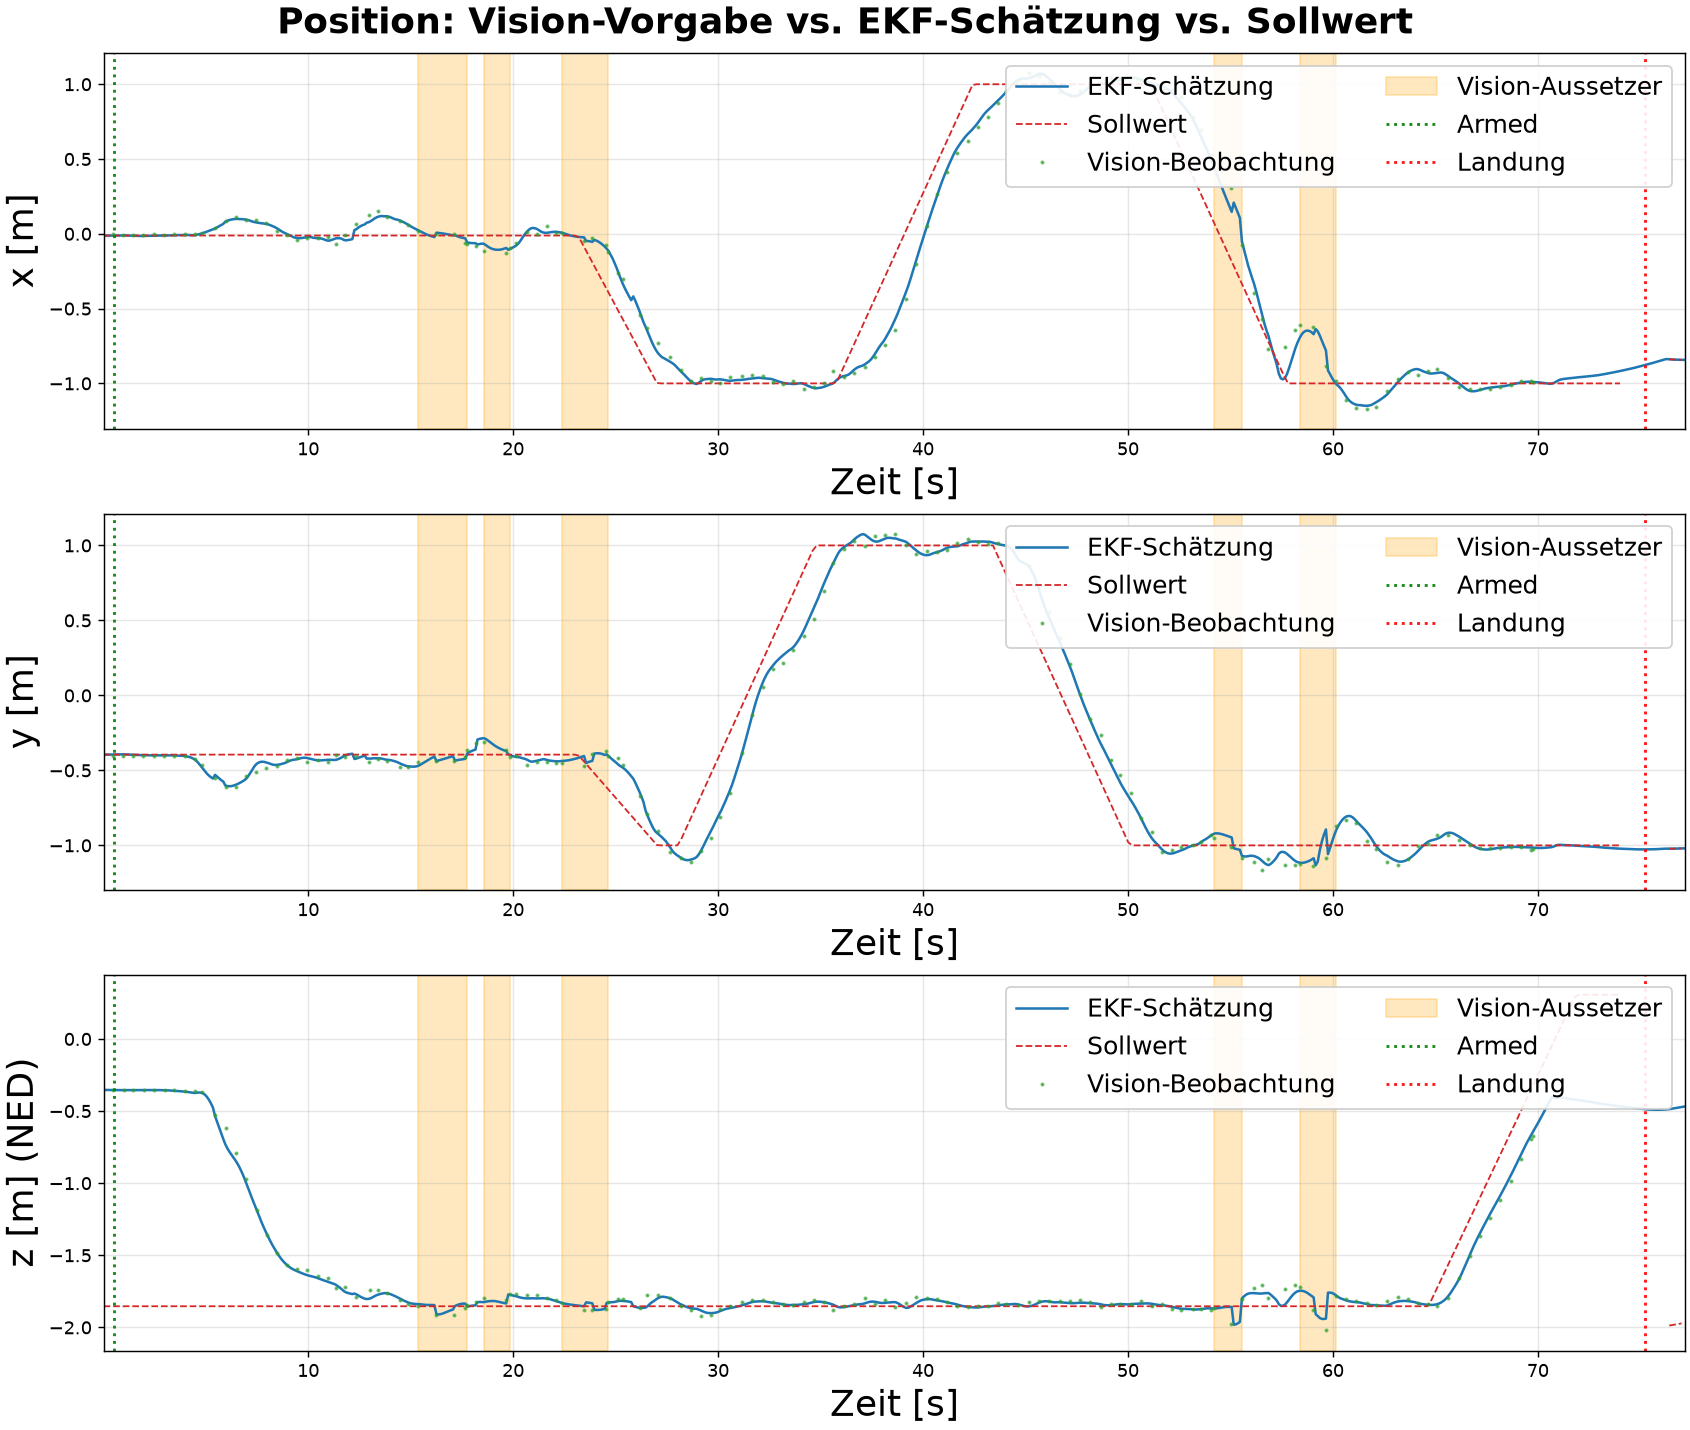
\includegraphics[width=1.0\textwidth]{Bilder/01_position_vision_ekf_sollwert.png}
\caption{Verlauf des aus den geloggten Positionswerten}
\label{fig:position_vision_ekf}
\end{figure}
\FloatBarrier
Abbildung~\ref{fig:position_vision_ekf} stellt die vom Begleitrechner eingespeiste Beobachtung, die Schätzung des \gls{ekf} und den Sollwert der Bahnführung einander gegenüber.
Die Vision-Beobachtungen erscheinen als Punkte in einem Raster von 2~Hz.
Dies ist keine Eigenschaft der Positionsbestimmung, sondern der Protokollierung, denn der Flugcontroller zeichnet die zugehörigen Topics nur mit dieser Rate auf.
Die tatsächliche Ausgaberate des Nodes beträgt wie zuvor erläutert 50~Hz.

Beobachtung und Schätzung liegen über den gesamten Flug hinweg praktisch deckungsgleich.
Der \gls{ekf} übernimmt die eingespeiste Pose also ohne erkennbare Verzerrung.
Der Sollwert wird im Schwebeflug eng gehalten, während im Demo-Modus ein Nachlauf gegenüber dem mit konstanter Geschwindigkeit wandernden Sollwert auftritt.
Dieser Nachlauf ist eine Eigenschaft der Bahnführung und keine Aussage über die Güte der Positionsbestimmung.

Die orange hinterlegten Bereiche kennzeichnen die Aussetzer der Vision-Stützung.
Ihre Verteilung folgt keinem Muster der Flugdynamik, denn die Lagewinkel bleiben über den gesamten Flug unterhalb von 3,2~Grad und unterscheiden sich vor den Aussetzern nicht von den Werten des ungestörten Reiseflugs.
Stattdessen sind die Aussetzer räumlich konzentriert.
Bei einer $y$-Position unterhalb von null rechnet der Zustandsschätzer je nach Bereich zwischen 4,6 und 16,9~Prozent der Zeit koppelnd, während oberhalb von null trotz eines Aufenthalts von knapp 16~s kein einziger Aussetzer auftritt.
Dies verweist auf eine Eigenschaft der Karte oder der Umgebung in diesem Bereich.
Die Ursache lässt sich aus dem Protokoll nicht abschließend bestimmen.







\section{Gesamtbewertung des Systems}
\label{sec:gesamtbewertung}
Dieser Abschnitt bewertet das Zusammenwirken der beiden Teilaufgaben Kartierung und Positionierung.
Zunächst wird die Kartierung, anschließend die Positionierung betrachtet.
Abschließend werden die Ergebnisse den in Abschnitt~\ref{sec:anforderungen} formulierten Anforderungen gegenübergestellt.

\subsection*{Bewertung der Kartierung}
\label{subsec:bewertung_kartierung}
Die Kartierung erfüllt ihre Aufgabe, aus einer handgeführten Aufnahme eine für die Positionsbestimmung nutzbare Karte zu erzeugen.
Alle drei Versuche liefern eine Karte ohne grobe Fehler, deren mittlerer räumlicher Abstand zur Sollkarte zwischen 9,57~mm und 12,75~mm liegt.
Von den 97 aufgebrachten Markern sind in jeder Karte 96 enthalten.
Der fehlende Eckmarker geht nicht auf das Verfahren, sondern auf eine unvollständige Aufzeichnung zurück und lässt sich durch eine sorgfältigere Kameraführung vermeiden.
Damit ist die in Abschnitt~\ref{sec:anforderungen} geforderte Karte der Versuchsumgebung gegeben, anhand derer sich die Position des \gls{uav}s im Weltkoordinatensystem bestimmen lässt.

Als tragfähig erweist sich das zweistufige Vorgehen aus Versuch~1 und Versuch~2.
Der erste Versuch liefert ohne jedes Vorwissen über die Kartengeometrie innerhalb von etwa 45~min eine Startschätzung, der zweite verfeinert diese unter Einbringen von Wissen über die Karte innerhalb von etwa zwei Stunden.
Der Betriebsmodus \texttt{slow} aus Versuch~3 rechtfertigt den vierfachen Rechenaufwand nicht, da er den mittleren räumlichen Abstand um lediglich 0,41~mm senkt und den Maximalwert sogar leicht anhebt.
Die Güte der Karte wird damit weniger durch die Rechenzeit als durch das eingebrachte Vorwissen bestimmt.
Bei der Aufzeichnung weiterer Karten sollte daher sämtliches verfügbare Wissen über die Geometrie der Umgebung in die Parametrierung einfließen.

Aus diesem Vorgehen folgt zugleich die geforderte Erweiterbarkeit der Karte.
Dieselbe Parametrierung lässt sich sowohl auf eine bislang unbekannte Umgebung als auch auf die Ergänzung einer bestehenden Karte anwenden.
Bereits bekannte Markerlagen werden dabei als Startlage vorgegeben und über das zugehörige Rauschen an ihre vermessene Position gebunden, während die neu hinzugekommenen Fiducial-Marker frei geschätzt werden.
Der nutzbare Flugbereich kann somit durch Ausbringen weiterer Fiducial-Marker und eine erneute Aufnahme räumlich vergrößert werden.

Die wesentliche verbleibende Schwäche ist der mit dem Abstand zum Ursprung wachsende Positionsfehler von 7,39~mm/m bis 9,93~mm/m.
Da sich alle Fiducial-Marker allein anhand des Ursprungsmarkers optimieren, baut sich der Fehler über die gesamte Kartenausdehnung auf und begrenzt die Skalierbarkeit des Verfahrens.
Für größere Umgebungen ist dieser Anstieg der bestimmende Fehleranteil, weshalb dort zusätzliche vermessene Stützstellen vorzusehen sind.

Die Aussagekraft der Bewertung ist durch die verwendete Referenz begrenzt.
Als Ground Truth dient die digitale Konstruktion der Druckvorlage und nicht eine unabhängige Vermessung der ausgebrachten Karte.
Der zwischen den Eckmarkern gemessene Versatz von etwa 5~mm zeigt, dass die physische Karte selbst von ihrer Sollgeometrie abweicht.
Die ausgewiesenen Abweichungen enthalten somit einen Anteil, der nicht der Kartierung, sondern dem Aufbringen der Klebefolie zuzurechnen ist.
Für die vorliegende Anwendung ist diese Genauigkeit ausreichend, da die Abweichungen deutlich unterhalb der im Flug auftretenden Positionsunsicherheit liegen.

Der Aufwand für die Kartierung bleibt gering und entspricht damit der Anforderung eines kostengünstigen Aufbaus.
Zur Aufnahme genügt eine handelsübliche \gls{usb}-Kamera und die Optimierung läuft auf gewöhnlicher Hardware.
Die eingesetzte Verarbeitungskette aus Detektion und Tag\gls{slam} ist quelloffen und frei verfügbar und über \gls{ros2} mit den übrigen Verarbeitungsschritten verbunden.

\subsection*{Bewertung der Positionierung}
\label{subsec:bewertung_positionierung}
Die Positionierung erfüllt die an sie gestellte Aufgabe.
Alle drei Flugversuche durchlaufen den festgelegten Ablauf aus Steigflug, Schwebeflug, Demo-Modus und Landung vollständig, ohne Eingriff über die Fernsteuerung.
Die Verarbeitungskette aus Bildaufnahme, Entzerrung, Markerdetektion, Positionsbestimmung und Übertragung an die Flugsteuerung arbeitet über die gesamte Flugdauer im geforderten Takt.
Der Zustandsschätzer übernimmt die eingespeiste Pose ohne erkennbare Verzerrung und verlässt die gestützte Navigation zu keinem Zeitpunkt.
Damit ist gezeigt, dass sich ein \gls{uav} allein anhand einer Markerkarte ohne Satellitennavigation im Innenraum führen lässt.
Die Anforderung, die Flugsteuerung durch \gls{px4} übernehmen zu lassen und ihr die extern berechnete Positionsschätzung zuzuführen, ist über die Anbindung mittels \gls{uxrce} erfüllt.

Auch die Positionierung ist vollständig aus quelloffener und frei verfügbarer Software aufgebaut und über \gls{ros2} als Softwaregrundlage miteinander verbunden.
Einschränkend ist anzumerken, dass die hardwarebeschleunigte Entzerrung und Markerdetektion über Isaac~ROS an die Jetson-Plattform gebunden ist.
Die Verarbeitungskette ist damit zwar quelloffen, aber nicht ohne Anpassung auf einen beliebigen Begleitrechner übertragbar.
Als Sensorik genügen zwei handelsübliche \gls{usb}-Kameras, sodass die Anforderung eines kostengünstigen Aufbaus im Flugbetrieb erfüllt bleibt.

Die Bewertung der Positionierung ist in ihrer Reichweite jedoch begrenzt.
Dem System steht keine von der Positionsbestimmung unabhängige Referenz der wahren Pose zur Verfügung, weshalb sich aus den Protokolldateien allein die Konsistenz der Fusion und nicht die absolute Genauigkeit ableiten lässt.
Alle folgenden Aussagen sind vor diesem Hintergrund zu lesen.

Aus demselben Grund lässt sich die Richtigkeit der extrinsischen Kalibrierung nicht nachweisen.
Für den Flugbetrieb ist ihre Genauigkeit allerdings von untergeordneter Bedeutung.
Für das Vorgehen ist eine Genauigkeit im unteren Millimeterbereich zu erwarten, da sie sich unmittelbar aus der von Hand vermessenen Lage der Tags und des Mittelpunkts ergeben.
Ein bewusst eingebrachter und deutlich größerer Kalibrierfehler blieb in Versuchen zudem ohne erkennbare Auswirkung auf das Flugverhalten.
Eine Abweichung im Montagewinkel der Kamera wirkt sich unmittelbar auf den Nickwinkel aus, der zur Positionsbestimmung des Zustandsschätzers nicht herangezogen wird.
Ein Kalibrierfehler in dieser Größe bleibt für die Flugführung damit weitgehend folgenlos.

Im Flug zeigt das \gls{uav} ein leichtes Schlingern um die Sollposition.
Diese Beobachtung ist qualitativer Natur und lässt sich aus den Protokolldateien nur bedingt belegen.
Als Ursache wird die konservativ angesetzte Standardabweichung der Vision-Stützung vermutet.
Der Parameter \texttt{EKF2\_EVP\_NOISE} gibt nach Abschnitt~\ref{subsec:kalman_gain} eine Standardabweichung von 0,1~m vor, die der Zustandsschätzer wegen \texttt{EKF2\_EV\_NOISE\_MD\,= 1} für jede Messung unverändert ansetzt.
In diese angenommene Unsicherheit geht neben der Streuung der Markerdetektion die Karte selbst ein, die nach Abschnitt~\ref{subsec:bewertung_kartierung} nicht fehlerfrei ist.
Ihre Fiducial-Marker weichen im Mittel um rund 10~mm und im Einzelfall um bis zu etwa 22~mm von der Sollkarte ab, wobei ein Teil dieser Abweichung bereits beim Aufbringen der Klebefolie entsteht.
Da sich die Pose des \gls{uav}s auf diese Markerlagen stützt, überträgt sich der Kartenfehler unmittelbar auf die eingespeiste Position.
Die Summe aus Detektions- und Kartenfehler dürfte gleichwohl deutlich unterhalb der angesetzten 0,1~m liegen, sodass die Messung gegenüber der Prädiktion zu schwach gewichtet wird und die Schätzung der eingespeisten Pose nur träge folgt.
Eine Bestimmung der tatsächlichen Streuung und eine daran ausgerichtete Parametrierung sind daher der naheliegende Ansatz zur Verbesserung des Flugverhaltens.

Eine weitere Einschränkung betrifft den nutzbaren Flugraum.
Das \gls{uav} kann sich nur innerhalb desjenigen Bereichs bewegen, in dem die Bodenkamera hinreichend viele Fiducial-Marker der Karte erfasst.
Der am Boden abgebildete Ausschnitt des Sichtfelds verschiebt sich bei einer Auslenkung um die Roll- und die Nickachse umso stärker, je größer der Abstand zur Karte ist.
Mit steigender Flughöhe gerät die vergleichsweise kleine Karte bei gleicher Lagewinkelauslenkung daher schneller aus dem Sichtfeld.
Nach unten ist der Flugraum ebenso begrenzt, da die Fiducial-Marker unterhalb einer bestimmten Höhe nicht mehr vollständig im Bild liegen.
Dies zeigt sich im Versuch bei der Landung, ab der die Positionsbestimmung bis zum Aufsetzen ausfällt.
Der zulässige Flugraum ist damit nach oben durch die Ausdehnung der Karte von 5,0~m~$\times$~3,9~m und nach unten durch die Markergrößen begrenzt.
Die Markeranordnung ist auf eine Mindestflughöhe von 1~m ausgelegt.

Der geforderte sichere Betrieb ist über mehrere unabhängige Ebenen abgedeckt.
Über die Fernsteuerung kann jederzeit in den Flug eingegriffen, in den Modus \texttt{Auto.Land} gewechselt oder über den Notausschalter abgeschaltet werden.
Bei Verlust der Verbindung zur Fernsteuerung oder zum Positionierungs-Node landet das \gls{uav} selbstständig.
Im Versuch war ein kein Eingriff über eine dieser Ebenen erforderlich.




